% =====================================================================
%  ĐỒ ÁN MÔN HỌC: DỮ LIỆU LỚN (BIG DATA)
%  Đề tài: Hệ thống gợi ý sản phẩm Software trên Amazon
%  Biên dịch bằng XeLaTeX (font Times New Roman)
% =====================================================================
\documentclass[12pt,a4paper]{report}

\usepackage{fontspec}
\defaultfontfeatures{Ligatures=TeX}
\setmainfont{Times New Roman}[
    Ligatures=TeX,
    Renderer=Basic,
]
\XeTeXgenerateactualtext=1

\usepackage[vietnamese]{babel}
\usepackage{xcolor}
\definecolor{textcolor}{RGB}{0,0,0}
\usepackage{graphicx}
\usepackage{adjustbox}
\usepackage{float}
\usepackage{amsmath}
\usepackage{amssymb}
\usepackage{booktabs}
\usepackage{multirow}
\usepackage{array}
\usepackage{longtable}
\usepackage{tabularx}
\usepackage{setspace}
\usepackage{placeins}
\usepackage{indentfirst}
\usepackage{enumitem}
\usepackage{listings}
\usepackage{caption}
\usepackage{subcaption}
\usepackage{tocloft}
\usepackage{geometry}
\usepackage{hyperref}

% ---------------------------------------------------------------------
% Highlight code (light theme kiểu GitHub)
% ---------------------------------------------------------------------
\definecolor{codekeyword}{RGB}{0,82,204}
\definecolor{codestring}{RGB}{196,26,22}
\definecolor{codecomment}{RGB}{98,98,98}
\definecolor{codebg}{RGB}{246,248,251}
\definecolor{codeborder}{RGB}{208,215,222}
\definecolor{codeplain}{RGB}{36,41,47}

\lstdefinestyle{codeLight}{
  basicstyle=\ttfamily\footnotesize,
  numbers=left,
  numberstyle=\tiny\color{codecomment},
  numbersep=8pt,
  showstringspaces=false,
  columns=fullflexible,
  keepspaces=true,
  breaklines=true,
  breakatwhitespace=true,
  postbreak=\mbox{\textcolor{codecomment}{\scriptsize$\hookrightarrow$}\space},
  tabsize=2,
  backgroundcolor=\color{codebg},
  frame=single,
  rulecolor=\color{codeborder},
  framesep=6pt,
  xleftmargin=14pt,
  framexleftmargin=10pt,
  keywordstyle=\bfseries\color{codekeyword},
  commentstyle=\itshape\color{codecomment},
  stringstyle=\color{codestring},
  literate=
    {á}{{\'a}}1 {à}{{\`a}}1 {ả}{{\h{a}}}1 {ã}{{\~a}}1 {ạ}{{\d{a}}}1
    {ă}{{\u{a}}}1 {â}{{\^a}}1 {đ}{{\dj}}1 {é}{{\'e}}1 {è}{{\`e}}1
    {ê}{{\^e}}1 {í}{{\'i}}1 {ì}{{\`i}}1 {ó}{{\'o}}1 {ò}{{\`o}}1
    {ô}{{\^o}}1 {ơ}{{\horn{o}}}1 {ú}{{\'u}}1 {ù}{{\`u}}1 {ư}{{\horn{u}}}1
    {ý}{{\'y}}1
}
\lstset{style=codeLight}

% ---------------------------------------------------------------------
% TikZ cho sơ đồ kiến trúc
% ---------------------------------------------------------------------
\usepackage{tikz}
\usetikzlibrary{shapes.geometric, arrows.meta, positioning, calc,
  decorations.pathreplacing, fit, backgrounds}
\tikzset{every node/.append style={align=center, inner sep=3pt}}

% ---------------------------------------------------------------------
% Caption: "Hình x.x" và "Bảng x.x" in nghiêng
% ---------------------------------------------------------------------
\DeclareCaptionLabelFormat{italiclabel}{\textit{#1~#2}}
\captionsetup[figure]{labelformat=italiclabel}
\captionsetup[table]{labelformat=italiclabel}

% ---------------------------------------------------------------------
% Trang trí & khoảng cách
% ---------------------------------------------------------------------
\emergencystretch=2em
\geometry{left=3cm, right=2cm, top=2cm, bottom=2cm}
\setstretch{1.15}

\makeatletter
\renewcommand\normalsize{\@setfontsize\normalsize{13pt}{18pt}}
\makeatother

\setlength{\parindent}{1.5em}
\setlength{\parskip}{0pt}

\makeatletter
\@afterindentfalse
% Giảm khoảng cách trước chapter heading
\renewcommand{\@makechapterhead}[1]{%
  \vspace*{-10pt}%
  {\parindent \z@ \raggedright \normalfont
    \ifnum \c@secnumdepth >\m@ne
        \Large\bfseries \@chapapp\space \thechapter
        \par\nobreak \vskip 4pt
    \fi
    \interlinepenalty\@M
    \huge \bfseries #1\par\nobreak \vskip 12pt
  }}
\renewcommand{\@makeschapterhead}[1]{%
  \vspace*{-10pt}%
  {\parindent \z@ \raggedright \normalfont
    \huge \bfseries #1\par\nobreak \vskip 12pt
  }}
\makeatother

\hypersetup{
    colorlinks=true,
    linkcolor=black,
    citecolor=black,
    filecolor=magenta,
    urlcolor=blue,
    pdftitle={Hệ thống gợi ý sản phẩm Software trên Amazon},
    pdfauthor={Đào Minh Trí},
}

\graphicspath{{images/}}

% Mục lục màu đen
\renewcommand{\cftfigfont}{\color{black}}
\renewcommand{\cfttabfont}{\color{black}}

\begin{document}
\color{textcolor}
\selectfont

% =====================================================================
%  TRANG BÌA
% =====================================================================
% =====================================================================
%  TRANG BÌA
% =====================================================================
\begin{titlepage}
\thispagestyle{empty}
\newgeometry{left=2.5cm, right=2.5cm, top=2cm, bottom=2cm}

% Khung viền trang bìa
\begin{tikzpicture}[remember picture,overlay]
    \draw[line width=1.2pt,color=blue!55]
        ([xshift=1.6cm,yshift=-1.5cm]current page.north west)
        rectangle
        ([xshift=-1.6cm,yshift=1.5cm]current page.south east);
    \draw[line width=0.6pt,color=blue!40]
        ([xshift=1.8cm,yshift=-1.7cm]current page.north west)
        rectangle
        ([xshift=-1.8cm,yshift=1.7cm]current page.south east);
\end{tikzpicture}

\begin{center}
    {\bfseries\large ĐẠI HỌC QUỐC GIA THÀNH PHỐ HỒ CHÍ MINH\\[4pt]
    TRƯỜNG ĐẠI HỌC CÔNG NGHỆ THÔNG TIN\\[4pt]
    KHOA KHOA HỌC VÀ KỸ THUẬT THÔNG TIN}\\[6pt]

    \begin{tikzpicture}
        \draw[line width=0.6pt,color=blue!50] (-1.6,0) -- (-0.35,0);
        \draw[line width=0.6pt,color=blue!50] (0.35,0) -- (1.6,0);
        \filldraw[fill=blue!50,draw=blue!50] (0,0) circle (2.2pt);
    \end{tikzpicture}

    \vspace{0.9cm}
    % --- Logo Trường Đại học Công nghệ Thông tin (UIT) ---
    
\includegraphics[width=0.30\textwidth]{uit_logo.pdf}

    \vspace{0.9cm}
    {\large ĐỒ ÁN MÔN HỌC: DỮ LIỆU LỚN (BIG DATA)}\\[1.0cm]

    {\setstretch{1.3}\Huge\bfseries
    HỆ THỐNG GỢI Ý SẢN PHẨM\\[6pt]
    SOFTWARE TRÊN AMAZON\par}

    \vspace{0.5cm}
    {\large\itshape Kiến trúc hai tháp (Two-Tower) với mô hình ngôn ngữ\\
    và học tương phản trên nền tảng dữ liệu lớn}\\[1.2cm]

    \renewcommand{\arraystretch}{1.5}
    \begin{tabular}{r l}
        \textbf{Giảng viên hướng dẫn:} & Phạm Huy Thanh \\
        \textbf{Sinh viên thực hiện:}  & Đào Minh Trí \\
        \textbf{Mã số sinh viên:}      & \dotfill{} \\
        \textbf{Lớp:}                  & \dotfill{} \\
    \end{tabular}
\end{center}

\vfill
\begin{center}
    {\bfseries TP. Hồ Chí Minh, tháng 6 năm 2026}
\end{center}

\end{titlepage}
\restoregeometry


% =====================================================================
%  PHẦN ĐẦU (không đánh số trang)
% =====================================================================
\pagenumbering{gobble}
% =====================================================================
%  LỜI CẢM ƠN
% =====================================================================
\newpage
\thispagestyle{plain}
\vspace*{0.5cm}
\begin{center}
    {\LARGE\textbf{\MakeUppercase{Lời cảm ơn}}}
\end{center}
\vspace{0.4cm}

Trước tiên, em xin gửi lời cảm ơn chân thành và sâu sắc nhất đến thầy
\textbf{Phạm Huy Thanh}, giảng viên hướng dẫn môn \textit{Dữ liệu lớn (Big Data)}.
Thầy đã tận tình truyền đạt những kiến thức nền tảng về hệ sinh thái xử lý
dữ liệu phân tán, đồng thời định hướng và góp ý chi tiết trong suốt quá trình
em thực hiện đồ án này. Những phản hồi quý báu của thầy giúp em hiểu rõ hơn
mối liên hệ giữa lý thuyết hệ thống gợi ý và bài toán xử lý dữ liệu quy mô lớn
trong thực tế.

\vspace{0.25cm}
Em cũng xin cảm ơn Trường Đại học Công nghệ Thông tin - Đại học Quốc gia
Thành phố Hồ Chí Minh và Khoa Khoa học và Kỹ thuật Thông tin đã tạo điều kiện
về môi trường học tập, tài nguyên tính toán và nguồn học liệu phong phú để em
có thể hoàn thành đồ án.

\vspace{0.25cm}
Do kiến thức và kinh nghiệm còn hạn chế, đồ án khó tránh khỏi những thiếu sót.
Em rất mong nhận được sự góp ý của thầy và các bạn để báo cáo được hoàn thiện hơn.

\vspace{0.25cm}
Em xin chân thành cảm ơn!

\vspace{0.8cm}
\begin{flushright}
    \begin{minipage}{0.6\textwidth}
        \centering
        TP. Hồ Chí Minh, tháng 6 năm 2026\\[0.2cm]
        \textit{Sinh viên thực hiện}\\[1.8cm]
        \textbf{Đào Minh Trí}
    \end{minipage}
\end{flushright}

% =====================================================================
%  TÓM TẮT
% =====================================================================
\newpage
\thispagestyle{plain}
\vspace*{0.5cm}
\begin{center}
    {\LARGE\textbf{\MakeUppercase{Tóm tắt đồ án}}}
\end{center}
\vspace{0.4cm}

Báo cáo trình bày quá trình thiết kế và xây dựng một \textbf{hệ thống gợi ý
(Recommender System)} cho nhóm sản phẩm \textit{Software} trên sàn thương mại điện
tử Amazon, đặt trong bối cảnh \textbf{dữ liệu lớn (Big Data)}. Khác với các hệ thống
lọc cộng tác truyền thống dựa trên định danh -- vốn bỏ qua văn bản ngữ nghĩa và gặp
khó với bài toán khởi động lạnh -- đồ án đề xuất một hướng tiếp cận hiện đại kết hợp
\textbf{mô hình ngôn ngữ}, \textbf{kiến trúc hai tháp (Two-Tower)} và \textbf{học
tương phản (contrastive learning)}.

\vspace{0.25cm}
Toàn bộ pipeline tiền xử lý được triển khai trên \textbf{Apache Spark (PySpark)}:
nạp dữ liệu Amazon Reviews thô, làm sạch, ghép nối các tập chia theo thời gian và
dựng văn bản ngữ nghĩa (\texttt{semantic\_text}) cho hơn $17.000$ sản phẩm, lưu trữ
tối ưu bằng định dạng cột \textbf{Parquet}. Mỗi sản phẩm được mã hóa thành vector
$384$ chiều bằng mô hình \texttt{all-MiniLM-L6-v2} (đóng băng); vector lịch sử của
$146.000$ người dùng được tổng hợp với \textbf{trọng số thời gian} kết hợp độ gần
đây và mức độ ưa thích. Mô hình hai tháp được huấn luyện bằng hàm mất mát
\textbf{InfoNCE} với mẫu âm trong batch, tối ưu bằng AdamW và tính toán độ chính xác
hỗn hợp trên GPU.

\vspace{0.25cm}
Hệ thống được đánh giá bằng giao thức \textbf{toàn kho (full-catalog)} khắt khe --
mã hóa trước toàn bộ kho sản phẩm rồi để mỗi người dùng cạnh tranh trên toàn bộ kho.
Kết quả cho thấy mô hình đạt Recall@10 $= 0{,}0142$ và Recall@50 $= 0{,}0436$,
\textbf{vượt trội hơn $24$ lần ở Top-$10$ và hơn $14$ lần ở Top-$50$} so với baseline
chọn ngẫu nhiên, đồng thời hội tụ ổn định mà không quá khớp. Báo cáo kết luận bằng
việc chỉ ra hạn chế của tháp sản phẩm đóng băng và đề xuất hướng phát triển: tinh
chỉnh tháp sản phẩm bằng LoRA và tích hợp tìm kiếm vector siêu tốc FAISS cho gợi ý
thời gian thực.

\vspace{0.4cm}
\noindent\textbf{Từ khóa:} \textit{Hệ thống gợi ý, Two-Tower, Mô hình ngôn ngữ,
Sentence Embedding, Học tương phản, InfoNCE, Apache Spark, Big Data, Amazon Reviews.}


\clearpage
\renewcommand{\contentsname}{MỤC LỤC}
\renewcommand{\listfigurename}{DANH SÁCH HÌNH VẼ}
\renewcommand{\listtablename}{DANH SÁCH BẢNG}
\tableofcontents
\clearpage
\listoffigures
\clearpage
\listoftables
% =====================================================================
%  DANH MỤC TỪ VIẾT TẮT
% =====================================================================
\clearpage
\thispagestyle{plain}
\vspace*{0.2cm}
\begin{center}
    {\LARGE\textbf{\MakeUppercase{Danh mục từ viết tắt}}}
\end{center}
\vspace{0.35cm}

{\small
\renewcommand{\arraystretch}{1.18}
\noindent\begin{tabularx}{\textwidth}{@{}l l X@{}}
\toprule
\textbf{Viết tắt} & \textbf{Thuật ngữ đầy đủ} & \textbf{Ý nghĩa} \\
\midrule
RS       & Recommender System            & Hệ thống gợi ý \\
CF       & Collaborative Filtering       & Lọc cộng tác \\
LLM      & Large Language Model          & Mô hình ngôn ngữ lớn \\
NLP      & Natural Language Processing    & Xử lý ngôn ngữ tự nhiên \\
MLP      & Multi-Layer Perceptron        & Mạng perceptron đa tầng \\
BN       & Batch Normalization           & Chuẩn hóa theo batch \\
InfoNCE  & Info Noise-Contrastive Estimation & Hàm mất mát tương phản dùng trong đồ án \\
NCE      & Noise-Contrastive Estimation  & Ước lượng tương phản nhiễu \\
NDCG     & Normalized Discounted Cumulative Gain & Độ lợi tích lũy chiết khấu chuẩn hóa \\
AMP      & Automatic Mixed Precision     & Tính toán độ chính xác hỗn hợp \\
FP16     & Half Precision Floating Point & Số thực dấu phẩy động 16-bit \\
LoRA     & Low-Rank Adaptation           & Tinh chỉnh tham số hạng thấp \\
FAISS    & Facebook AI Similarity Search & Thư viện tìm kiếm vector tương đồng \\
EDA      & Exploratory Data Analysis     & Phân tích khám phá dữ liệu \\
GPU      & Graphics Processing Unit      & Bộ xử lý đồ họa \\
API      & Application Programming Interface & Giao diện lập trình ứng dụng \\
ASIN     & Amazon Standard Identification Number & Mã định danh sản phẩm trên Amazon \\
\bottomrule
\end{tabularx}
}


% =====================================================================
%  NỘI DUNG CHÍNH
% =====================================================================
\clearpage
\pagenumbering{arabic}
\setcounter{page}{1}

% =====================================================================
%  CHƯƠNG 1: TỔNG QUAN ĐỀ TÀI
% =====================================================================
\chapter{Tổng quan đề tài}
\label{chap:intro}

\section{Đặt vấn đề}

Thương mại điện tử hiện đại đặt người dùng trước hàng triệu lựa chọn, dẫn tới hiện
tượng \textit{quá tải thông tin} (information overload). \textbf{Hệ thống gợi ý}
(Recommender System) ra đời nhằm tự động lọc và đề xuất cho mỗi người dùng những sản
phẩm phù hợp nhất với sở thích của họ. Đối với nhóm sản phẩm \textbf{Software} (phần
mềm) trên Amazon, bài toán càng quan trọng bởi sản phẩm mang tính chuyên biệt cao,
mô tả kỹ thuật dài và đánh giá người dùng giàu ngữ nghĩa.

Tuy nhiên, các hệ thống gợi ý truyền thống dựa trên \textbf{định danh} (ID-based
collaborative filtering) bộc lộ hai hạn chế cố hữu:

\begin{itemize}[leftmargin=2em, itemsep=2pt]
    \item \textbf{Bỏ qua dữ liệu văn bản ngữ nghĩa:} các mô hình lọc cộng tác cổ
    điển chỉ học từ ma trận tương tác (ai đã mua/đánh giá gì), hoàn toàn không khai
    thác phần mô tả sản phẩm, tính năng hay nội dung review -- vốn chứa thông tin
    rất giá trị về bản chất sản phẩm.
    \item \textbf{Bài toán khởi động lạnh (cold-start):} khi xuất hiện người dùng
    mới hoặc sản phẩm mới chưa có lịch sử tương tác, mô hình dựa trên định danh không
    thể đưa ra dự đoán đáng tin cậy.
\end{itemize}

\section{Giải pháp đề xuất}

Đồ án đề xuất một hướng tiếp cận hiện đại nhằm khắc phục đồng thời hai hạn chế trên,
dựa trên ba trụ cột:

\begin{enumerate}[leftmargin=2em, itemsep=2pt]
    \item \textbf{Mô hình ngôn ngữ (Language Model):} sử dụng một mô hình ngôn ngữ
    dựa trên kiến trúc Transformer để \textit{hiểu} văn bản mô tả sản phẩm và nội
    dung đánh giá, chuyển toàn bộ thông tin văn bản dài thành một \textit{vector số
    cố định} đại diện cho ý nghĩa của sản phẩm. Nhờ vậy, hệ thống nắm bắt được sự
    tương đồng ngữ nghĩa ngay cả với sản phẩm mới.
    \item \textbf{Kiến trúc hai tháp (Two-Tower):} tách riêng việc biểu diễn
    \textit{người dùng} và \textit{sản phẩm} thành hai nhánh độc lập, cùng ánh xạ
    vào một không gian vector chung. Nhánh người dùng học từ \textit{chuỗi hành vi
    theo thời gian}, có tính tới yếu tố thời điểm và mức độ ưa thích.
    \item \textbf{Học tương phản (Contrastive Learning):} huấn luyện mô hình bằng
    cách kéo các sản phẩm mà người dùng thích lại gần vector người dùng và đẩy các
    sản phẩm không liên quan ra xa trong không gian biểu diễn.
\end{enumerate}

\section{Mục tiêu và phạm vi}

\textbf{Mục tiêu} của đồ án là xây dựng một \textit{luồng xử lý hoàn chỉnh}
(end-to-end pipeline) cho hệ thống gợi ý phần mềm, bao gồm:

\begin{itemize}[leftmargin=2em, itemsep=2pt]
    \item Nạp và tiền xử lý dữ liệu lớn bằng \textbf{Apache Spark}, lưu trữ tối ưu
    theo định dạng cột \textbf{Apache Parquet}.
    \item Mã hóa "trải nghiệm" của người dùng thành vector bằng mô hình ngôn ngữ,
    tích hợp trọng số thời gian.
    \item Huấn luyện mô hình hai tháp với hàm mất mát tương phản.
    \item Đánh giá khách quan độ hiệu quả trên \textbf{toàn bộ kho sản phẩm}
    (full-catalog), thay vì chỉ trên một nhóm nhỏ.
\end{itemize}

\textbf{Phạm vi:} Báo cáo tập trung vào danh mục \textit{Software} của bộ dữ liệu
Amazon Reviews 2023, với khoảng $146.000$ người dùng và hơn $17.000$ sản phẩm phần
mềm độc nhất. Bài toán được mô hình hóa theo dạng \textbf{truy hồi} (retrieval):
với mỗi người dùng, hệ thống xếp hạng toàn bộ kho sản phẩm và trả về danh sách
Top-$N$ phù hợp nhất.

\section{Đóng góp của báo cáo}

\begin{itemize}[leftmargin=2em, itemsep=2pt]
    \item Xây dựng pipeline xử lý dữ liệu lớn end-to-end trên PySpark, tạo ra biểu
    diễn văn bản ngữ nghĩa (\texttt{semantic\_text}) thống nhất cho sản phẩm.
    \item Thiết kế thuật toán tổng hợp vector lịch sử người dùng có \textit{trọng số
    thời gian} (recency) kết hợp mức độ ưa thích (rating), tính toán hiệu quả trên
    bộ nhớ.
    \item Cài đặt và huấn luyện mô hình Two-Tower với mô hình ngôn ngữ làm bộ mã hóa
    sản phẩm và hàm mất mát tương phản InfoNCE.
    \item Đề xuất giao thức đánh giá \textbf{full-catalog} loại bỏ thiên lệch đánh
    giá cục bộ, chứng minh mô hình vượt trội nhiều lần so với baseline ngẫu nhiên.
\end{itemize}

\section{Cấu trúc báo cáo}

Báo cáo được tổ chức theo năm chương:

\begin{itemize}[leftmargin=2em, itemsep=2pt]
    \item \textbf{Chương 1 -- Tổng quan đề tài:} đặt vấn đề, giải pháp, mục tiêu và
    phạm vi.
    \item \textbf{Chương 2 -- Cơ sở lý thuyết:} nền tảng dữ liệu lớn, mô hình ngôn
    ngữ, kiến trúc hai tháp và học tương phản.
    \item \textbf{Chương 3 -- Phân tích và thiết kế hệ thống:} kiến trúc tổng thể,
    xử lý dữ liệu, chiến lược chia dữ liệu và thiết kế mô hình.
    \item \textbf{Chương 4 -- Kết quả thực nghiệm:} môi trường, giao thức đánh giá
    và phân tích kết quả.
    \item \textbf{Chương 5 -- Kết luận và hướng phát triển:} tổng kết, hạn chế và
    định hướng tương lai.
\end{itemize}

% =====================================================================
%  CHƯƠNG 2: CƠ SỞ LÝ THUYẾT
% =====================================================================
\chapter{Cơ sở lý thuyết}
\label{chap:background}

\section{Hệ thống gợi ý theo hướng truy hồi}

Gọi tập người dùng là $U$ và tập sản phẩm là $I$. Thay vì dự đoán điểm số cho từng
cặp như lọc cộng tác cổ điển, đồ án mô hình hóa bài toán theo hướng \textbf{truy hồi
dựa trên biểu diễn} (embedding-based retrieval): mỗi người dùng $u$ và mỗi sản phẩm
$i$ được ánh xạ thành các vector $\mathbf{u}, \mathbf{v} \in \mathbb{R}^d$ trong cùng
một không gian. Mức độ phù hợp được đo bằng độ tương đồng cosine:

\begin{equation}
    \text{score}(u, i) = \cos(\mathbf{u}, \mathbf{v})
    = \frac{\mathbf{u} \cdot \mathbf{v}}{\|\mathbf{u}\|\,\|\mathbf{v}\|}.
\end{equation}

Khi cả hai vector đã được chuẩn hóa $L_2$ (độ dài bằng $1$), độ tương đồng cosine
trở thành tích vô hướng đơn giản. Gợi ý Top-$N$ chính là việc tìm $N$ sản phẩm có
score cao nhất với người dùng -- một bài toán \textit{tìm kiếm láng giềng gần nhất}
(nearest neighbor search) trong không gian vector, có thể tăng tốc bằng các thư viện
chuyên dụng. Hướng tiếp cận này là nền tảng của các hệ thống gợi ý công nghiệp quy
mô lớn nhờ khả năng tách biệt việc tính toán biểu diễn người dùng và sản phẩm.

\section{Các hướng nghiên cứu liên quan}

Lĩnh vực hệ thống gợi ý đã trải qua nhiều giai đoạn phát triển:

\begin{itemize}[leftmargin=2em, itemsep=2pt]
    \item \textbf{Lọc cộng tác cổ điển:} từ các phương pháp dựa trên láng giềng
    (user/item-based KNN) tới \textit{phân rã ma trận} (Matrix Factorization, ALS),
    học các nhân tố ẩn từ ma trận tương tác. Hạn chế chung là chỉ dùng tín hiệu định
    danh và gặp khó với cold-start.
    \item \textbf{Học sâu cho gợi ý:} các mô hình như Neural Collaborative Filtering
    thay tích vô hướng bằng mạng nơ-ron để học tương tác phi tuyến, song vẫn dựa trên
    embedding theo định danh.
    \item \textbf{Truy hồi hai tháp:} được phổ biến bởi các hệ thống công nghiệp quy
    mô lớn (YouTube, Google), kiến trúc hai tháp cho phép truy hồi ứng viên cực nhanh
    từ kho hàng triệu mục, thường huấn luyện bằng học tương phản với mẫu âm trong
    batch.
    \item \textbf{Gợi ý dựa trên ngôn ngữ:} xu hướng gần đây kết hợp mô hình ngôn
    ngữ để khai thác văn bản mô tả sản phẩm, giúp biểu diễn giàu ngữ nghĩa và giảm
    phụ thuộc vào lịch sử tương tác -- đặc biệt hữu ích cho cold-start.
\end{itemize}

Đồ án kế thừa và kết hợp hai hướng cuối: dùng \textit{mô hình ngôn ngữ} làm tháp sản
phẩm trong kiến trúc \textit{hai tháp}, huấn luyện bằng \textit{học tương phản} --
một thiết kế hiện đại, phù hợp với bối cảnh dữ liệu lớn và đặc thù giàu văn bản của
sản phẩm phần mềm.

\section{Nền tảng dữ liệu lớn}

\subsection{Apache Spark}

\textbf{Apache Spark} là nền tảng tính toán phân tán cho phép xử lý dữ liệu quy mô
lớn theo cơ chế song song trong bộ nhớ. Trong đồ án, Spark đảm nhận toàn bộ khâu
tiền xử lý nặng: nạp dữ liệu JSON/JSONL thô, khử trùng lặp, ghép nối (join) các tập
dữ liệu và biến đổi đặc trưng. API \texttt{DataFrame} cùng bộ tối ưu truy vấn
\textit{Catalyst} giúp các phép biến đổi được thực thi hiệu quả; kỹ thuật
\textbf{broadcast join} được dùng để ghép tập tương tác nhỏ với bảng dữ liệu lớn mà
không gây xáo trộn (shuffle) tốn kém.

\subsection{Định dạng cột Apache Parquet}

Sau tiền xử lý, dữ liệu được lưu dưới định dạng \textbf{Apache Parquet} -- một định
dạng lưu trữ \textit{theo cột} (columnar). So với định dạng dòng (CSV, JSON),
Parquet mang lại các ưu điểm then chốt cho dữ liệu lớn:

\begin{itemize}[leftmargin=2em, itemsep=2pt]
    \item \textbf{Nén hiệu quả:} dữ liệu cùng cột có kiểu giống nhau nên nén tốt,
    giảm đáng kể dung lượng lưu trữ.
    \item \textbf{Đọc chọn lọc:} chỉ cần đọc các cột liên quan, giảm I/O.
    \item \textbf{Tốc độ đọc/ghi cao:} phù hợp với các tác vụ phân tích và huấn
    luyện lặp lại.
\end{itemize}

Để tăng tốc độ nạp dữ liệu khi huấn luyện, đồ án áp dụng kỹ thuật \textbf{nạp dữ
liệu đa luồng bất đồng bộ} (asynchronous multi-worker loading) thông qua
\texttt{DataLoader}, cho phép phần cứng CPU chuẩn bị batch tiếp theo trong khi GPU
đang tính toán batch hiện tại.

\section{Mô hình ngôn ngữ và biểu diễn văn bản}

\subsection{Kiến trúc Transformer}

\textbf{Mô hình ngôn ngữ} hiện đại dựa trên kiến trúc \textbf{Transformer} với cơ
chế \textit{tự chú ý} (self-attention), cho phép mô hình nắm bắt mối quan hệ ngữ
nghĩa giữa các từ trong văn bản bất kể khoảng cách. Cơ chế chú ý tính trọng số liên
kết giữa các token dựa trên ba ma trận truy vấn (Query), khóa (Key) và giá trị
(Value):

\begin{equation}
    \text{Attention}(Q, K, V) = \text{softmax}\!\left(\frac{Q K^\top}{\sqrt{d_k}}\right) V,
\end{equation}

trong đó $d_k$ là số chiều của vector khóa, đóng vai trò hệ số tỷ lệ giúp ổn định
gradient. Mỗi tầng Transformer (Hình~\ref{fig:encoder}) gồm một khối \textit{chú ý
đa đầu} (multi-head attention) và một mạng \textit{truyền thẳng} (feed-forward),
mỗi khối kèm kết nối tắt (residual) và chuẩn hóa lớp (layer norm). MiniLM xếp chồng
$6$ tầng như vậy. Nhờ tính toán song song trên toàn bộ chuỗi, Transformer học được
biểu diễn ngữ cảnh phong phú.

\begin{figure}[H]
\centering
\begin{tikzpicture}[
    font=\scriptsize, node distance=0.45cm,
    blk/.style={rectangle, rounded corners=2pt, draw=blue!55, fill=blue!8,
        line width=0.7pt, text width=3.4cm, minimum height=0.6cm, align=center},
    an/.style={rectangle, rounded corners=2pt, draw=teal!55, fill=teal!10,
        line width=0.7pt, text width=3.4cm, minimum height=0.5cm, align=center},
    a/.style={-{Stealth[length=1.8mm]}, line width=0.6pt, blue!55}
]
\node[blk, fill=gray!10, draw=gray!55] (in) {Embedding token + vị trí};
\node[blk, above=of in] (mha) {Multi-Head\\Self-Attention};
\node[an, above=of mha] (an1) {Add \& LayerNorm};
\node[blk, above=of an1] (ffn) {Feed-Forward (FFN)};
\node[an, above=of ffn] (an2) {Add \& LayerNorm};
\node[blk, fill=gray!10, draw=gray!55, above=of an2] (out) {Biểu diễn ngữ cảnh};
\draw[a] (in)--(mha); \draw[a] (mha)--(an1); \draw[a] (an1)--(ffn);
\draw[a] (ffn)--(an2); \draw[a] (an2)--(out);
% residual arrows
\draw[a, gray!55, dashed] (in.east) -- ++(1.3,0) |- (an1.east);
\draw[a, gray!55, dashed] (an1.west) -- ++(-1.3,0) |- (an2.west);
\node[draw=blue!45, rounded corners=3pt, dashed, fit=(mha)(an1)(ffn)(an2),
      inner sep=5pt, label={[font=\scriptsize\bfseries, blue!55!black]right:$\times\,6$ tầng}] {};
\end{tikzpicture}
\caption{Cấu trúc một tầng mã hóa Transformer (MiniLM xếp chồng $6$ tầng)}
\label{fig:encoder}
\end{figure} Đồ án sử dụng mô hình \texttt{all-MiniLM-L6-v2} thuộc họ
\textit{Sentence-Transformers} -- một mô hình gọn nhẹ ($6$ tầng, đầu ra $384$ chiều,
khoảng $22{,}7$ triệu tham số) được chưng cất (distillation) và tinh chỉnh chuyên để
sinh \textbf{vector câu} (sentence embedding) chất lượng cao, cân bằng tốt giữa độ
chính xác và tốc độ -- phù hợp với yêu cầu mã hóa hàng trăm nghìn văn bản.

\subsection{Từ văn bản tới vector ngữ nghĩa}

Văn bản mô tả sản phẩm (tiêu đề, tính năng, mô tả, danh mục\ldots) được đưa qua mô
hình để thu các vector ngữ cảnh cho từng token. Để có một vector \textit{cố định}
đại diện cho toàn bộ văn bản, đồ án áp dụng phép \textbf{trung bình có mặt nạ}
(mean pooling) trên các token:

\begin{equation}
    \mathbf{v} = \frac{\sum_{t} m_t \, \mathbf{h}_t}{\sum_{t} m_t},
\end{equation}

với $\mathbf{h}_t$ là vector của token thứ $t$ và $m_t \in \{0, 1\}$ là mặt nạ chú ý
(loại bỏ token đệm). Vector kết quả được chuẩn hóa $L_2$. Nhờ vậy, hai sản phẩm có
mô tả tương đồng về ngữ nghĩa sẽ có vector gần nhau, giải quyết được vấn đề khởi động
lạnh cho sản phẩm mới.

\subsection{Tiền huấn luyện và Sentence-BERT}

Sức mạnh của bộ mã hóa đến từ quá trình \textbf{tiền huấn luyện} (pre-training) trên
kho văn bản khổng lồ, giúp mô hình tích lũy tri thức ngôn ngữ tổng quát trước khi áp
dụng cho bài toán cụ thể. Tuy nhiên, các vector token từ BERT gốc không tối ưu cho
việc đo độ tương đồng câu. \textbf{Sentence-BERT} khắc phục bằng cách tinh chỉnh mô
hình theo cặp/bộ ba câu với mục tiêu sao cho các câu cùng nghĩa có vector gần nhau --
chính là tinh thần của học tương phản. Mô hình \texttt{all-MiniLM-L6-v2} được huấn
luyện trên hơn một tỷ cặp câu, nên vector $384$ chiều mà nó sinh ra mang chất lượng
ngữ nghĩa cao, rất phù hợp để làm \textit{biểu diễn sản phẩm cố định} trong tháp Item.
Đây là lý do đồ án có thể \textbf{đóng băng} tháp này mà vẫn thu được không gian biểu
diễn tốt, tiết kiệm đáng kể tài nguyên huấn luyện.

\section{Kiến trúc hai tháp (Two-Tower)}
\label{sec:twotower}

\textbf{Two-Tower} (hay \textit{dual encoder}) là kiến trúc gồm hai nhánh mạng độc
lập (Hình~\ref{fig:twotower}): một \textbf{tháp sản phẩm} mã hóa sản phẩm và một
\textbf{tháp người dùng} mã hóa người dùng, cùng cho ra vector trong một không gian
chung. Điểm mạnh của kiến trúc này là hai tháp có thể tính toán \textit{tách rời}:
toàn bộ vector sản phẩm có thể được mã hóa trước (offline) và lập chỉ mục, còn vector
người dùng chỉ cần tính khi cần gợi ý -- nhờ vậy hệ thống truy hồi cực nhanh trên kho
sản phẩm lớn.

\begin{figure}[H]
\centering
\begin{tikzpicture}[
    node distance=0.5cm and 1.0cm,
    box/.style={rectangle, rounded corners=3pt, draw=blue!55, fill=blue!9,
        line width=0.8pt, text width=3.0cm, minimum height=0.8cm, font=\footnotesize},
    frozen/.style={rectangle, rounded corners=3pt, draw=gray!60, fill=gray!12,
        line width=0.8pt, text width=3.0cm, minimum height=0.8cm, font=\footnotesize},
    op/.style={circle, draw=teal!65, fill=teal!12, line width=0.9pt,
        minimum size=0.95cm, font=\small},
    arr/.style={-{Stealth[length=2mm]}, line width=0.7pt, blue!60}
]
% User tower (left)
\node[box] (uin) {Vector lịch sử người dùng (384-d)};
\node[box, above=of uin] (ump) {Tháp User: MLP\\$384{\to}512{\to}384$\\BatchNorm + Dropout};
\node[box, above=of ump] (unorm) {Chuẩn hóa $L_2$};
\draw[arr] (uin) -- (ump);
\draw[arr] (ump) -- (unorm);
% Item tower (right)
\node[frozen, right=2.4cm of uin] (iin) {Văn bản sản phẩm\\(semantic\_text)};
\node[frozen, above=of iin] (ienc) {Tháp Item: MiniLM\\(\textbf{đóng băng})\\+ mean pooling};
\node[frozen, above=of ienc] (inorm) {Chuẩn hóa $L_2$};
\draw[arr, gray!60] (iin) -- (ienc);
\draw[arr, gray!60] (ienc) -- (inorm);
% similarity
\node[op] (sim) at ($(unorm)!0.5!(inorm) + (0,1.2)$) {$\cos$};
\draw[arr] (unorm) -- (sim);
\draw[arr, gray!60] (inorm) -- (sim);
\node[above=0.35cm of sim, font=\footnotesize\bfseries, text=teal!50!black]
    {Độ tương đồng → Loss InfoNCE};
\end{tikzpicture}
\caption{Kiến trúc hai tháp (Two-Tower) với tháp sản phẩm đóng băng}
\label{fig:twotower}
\end{figure}

Trong thiết kế của đồ án, \textbf{tháp sản phẩm được đóng băng hoàn toàn} (không cập
nhật trọng số) nhằm tiết kiệm bộ nhớ và tận dụng tri thức ngôn ngữ sẵn có; chỉ
\textbf{tháp người dùng} (một mạng nơ-ron đa tầng) được huấn luyện để học cách ánh
xạ lịch sử hành vi sang không gian sản phẩm.

\section{Học tương phản và hàm mất mát InfoNCE}
\label{sec:infonce}

\textbf{Học tương phản} (Contrastive Learning) huấn luyện mô hình bằng cách so sánh:
với mỗi người dùng, sản phẩm thực sự tương tác (mẫu dương) cần được kéo lại gần,
trong khi các sản phẩm khác (mẫu âm) bị đẩy ra xa. Đồ án sử dụng hàm mất mát
\textbf{InfoNCE} với chiến lược \textit{mẫu âm trong batch} (in-batch negatives):
trong một batch gồm $B$ cặp (người dùng, sản phẩm), sản phẩm của các cặp còn lại
đóng vai trò mẫu âm cho người dùng đang xét. Hàm mất mát cho người dùng $i$ là:

\begin{equation}
    \mathcal{L}_i = -\log
    \frac{\exp\!\big(\cos(\mathbf{u}_i, \mathbf{v}_i)/\tau\big)}
         {\sum_{j=1}^{B} \exp\!\big(\cos(\mathbf{u}_i, \mathbf{v}_j)/\tau\big)},
\end{equation}

trong đó $\mathbf{v}_i$ là sản phẩm dương của người dùng $i$, $\mathbf{v}_j$ là các
sản phẩm trong batch, và $\tau$ là \textit{tham số nhiệt độ} (temperature) điều
chỉnh độ "sắc" của phân phối. Về bản chất, đây là một bài toán phân loại $B$ lớp mà
nhãn đúng nằm trên đường chéo của ma trận tương đồng -- cài đặt hiệu quả bằng
\texttt{CrossEntropyLoss}. Chiến lược in-batch negatives giúp tận dụng tối đa mỗi
batch mà không cần lấy mẫu âm tường minh, rất phù hợp với huấn luyện quy mô lớn.
Hình~\ref{fig:infonce} minh họa trực quan: ma trận tương đồng $B \times B$ giữa mọi
người dùng và mọi sản phẩm trong batch, trong đó nhiệm vụ huấn luyện là làm cho các
ô \textit{đường chéo} (cặp đúng) có giá trị cao nhất trên mỗi hàng.

\begin{figure}[H]
\centering
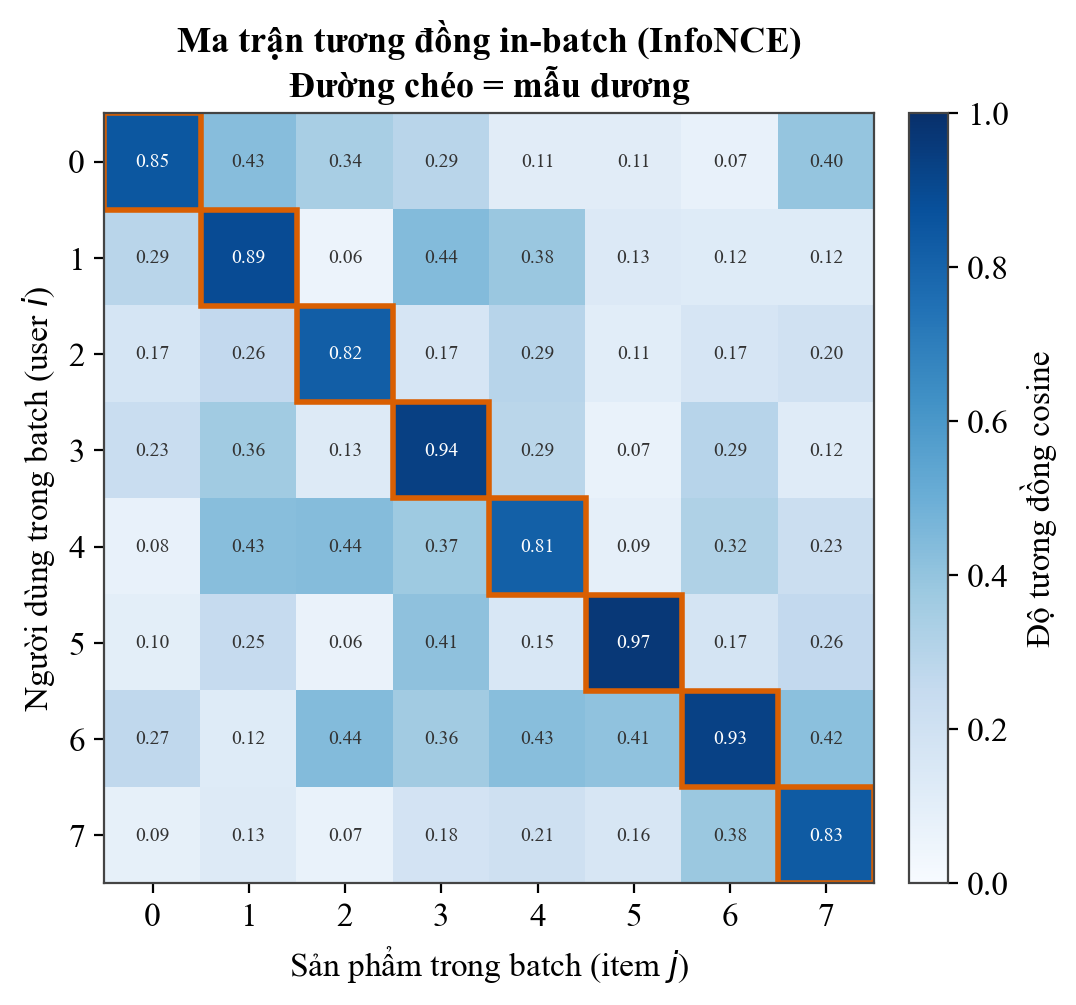
\includegraphics[width=0.58\textwidth]{infonce_matrix.png}
\caption{Ma trận tương đồng in-batch của InfoNCE; đường chéo là cặp dương cần tối đa hóa}
\label{fig:infonce}
\end{figure}

\subsection{Vai trò của tham số nhiệt độ}

Tham số nhiệt độ $\tau$ kiểm soát mức độ "gay gắt" của hàm mất mát. Khi $\tau$ nhỏ,
mô hình \textit{trừng phạt mạnh} những mẫu âm khó (nằm gần mẫu dương), thúc đẩy phân
tách rạch ròi trong không gian biểu diễn; khi $\tau$ lớn, gradient trải đều và mô
hình "khoan dung" hơn. Về mặt lý thuyết, học tương phản tối ưu đồng thời hai tính
chất: \textbf{alignment} (các cặp dương phải gần nhau) và \textbf{uniformity} (các
biểu diễn phải trải đều trên mặt cầu đơn vị để giữ nhiều thông tin). Giá trị
$\tau = 0{,}1$ được đồ án lựa chọn là một mức cân bằng phổ biến và hiệu quả cho bài
toán gợi ý.

\section{Tìm kiếm láng giềng gần nhất}
\label{sec:ann}

Sau khi huấn luyện, việc gợi ý Top-$N$ quy về tìm các sản phẩm có vector gần vector
người dùng nhất. Với kho chỉ vài chục nghìn sản phẩm, ta có thể tính tương đồng
\textit{vét cạn} (brute-force) như trong giao thức đánh giá của đồ án. Tuy nhiên, khi
kho lên tới hàng triệu sản phẩm, phép vét cạn trở nên quá tốn kém cho yêu cầu thời
gian thực. Khi đó, các kỹ thuật \textbf{tìm kiếm láng giềng gần nhất xấp xỉ}
(Approximate Nearest Neighbor -- ANN) như chỉ mục đảo (IVF), lượng tử hóa tích
(product quantization) hay đồ thị HNSW -- được hiện thực trong thư viện
\textbf{FAISS} -- cho phép truy hồi trong vài phần nghìn giây với độ chính xác gần
như không suy giảm. Kiến trúc hai tháp đặc biệt phù hợp với ANN vì toàn bộ vector
sản phẩm có thể được lập chỉ mục trước. Đây là nền tảng cho hướng phát triển triển
khai thời gian thực ở Chương~\ref{chap:conclusion}.

\section{Các độ đo đánh giá}
\label{sec:metrics}

Vì bài toán là truy hồi Top-$N$, đồ án dùng hai độ đo xếp hạng phổ biến, tính trên
\textbf{toàn bộ kho sản phẩm}. Với mỗi người dùng, gọi $\text{Rel}_u$ là tập sản
phẩm thực sự liên quan và $\text{Rec}_u^K$ là Top-$K$ sản phẩm được gợi ý:

\begin{equation}
    \text{Recall@K} = \frac{|\text{Rec}_u^K \cap \text{Rel}_u|}{|\text{Rel}_u|}.
\end{equation}

Trong giao thức leave-one-out (mỗi người dùng có đúng một sản phẩm mục tiêu),
Recall@K rút gọn thành tỷ lệ người dùng có sản phẩm mục tiêu nằm trong Top-$K$.
\textbf{NDCG@K} bổ sung yếu tố thứ hạng, thưởng nhiều hơn khi sản phẩm đúng xuất hiện
ở vị trí cao:

\begin{equation}
    \text{NDCG@K} = \frac{1}{\log_2(p + 1)},
\end{equation}

với $p$ là vị trí của sản phẩm mục tiêu trong danh sách gợi ý (nếu nằm trong Top-$K$,
ngược lại bằng $0$). Việc đánh giá trên toàn kho $\sim 17.000$ sản phẩm khiến các
con số tuyệt đối nhỏ, nhưng phản ánh \textit{trung thực} độ khó thực tế và cho phép
so sánh công bằng với baseline chọn ngẫu nhiên.

\subsection{Toàn kho và thiên lệch lấy mẫu}
\label{sec:fullcatalog}

Nhiều nghiên cứu đánh giá theo cách \textit{lấy mẫu} (sampled metric): trộn sản phẩm
mục tiêu với một số ít mẫu âm (ví dụ $99$ hoặc $999$ sản phẩm) rồi xếp hạng trong
nhóm nhỏ đó. Cách này nhanh nhưng gây \textbf{thiên lệch lạc quan}: kho ứng viên càng
nhỏ, chỉ số càng cao một cách giả tạo. Hình~\ref{fig:evalproto} minh họa hiện tượng
này -- cùng một mô hình, Recall@10 giảm mạnh từ khoảng $0{,}42$ (chỉ $100$ ứng viên)
xuống $0{,}0142$ khi xếp hạng trên toàn bộ $17.000$ sản phẩm. Do đó, đồ án chủ trương
đánh giá \textbf{toàn kho (full-catalog)} để có con số trung thực, dù khắt khe hơn.

\begin{figure}[H]
\centering
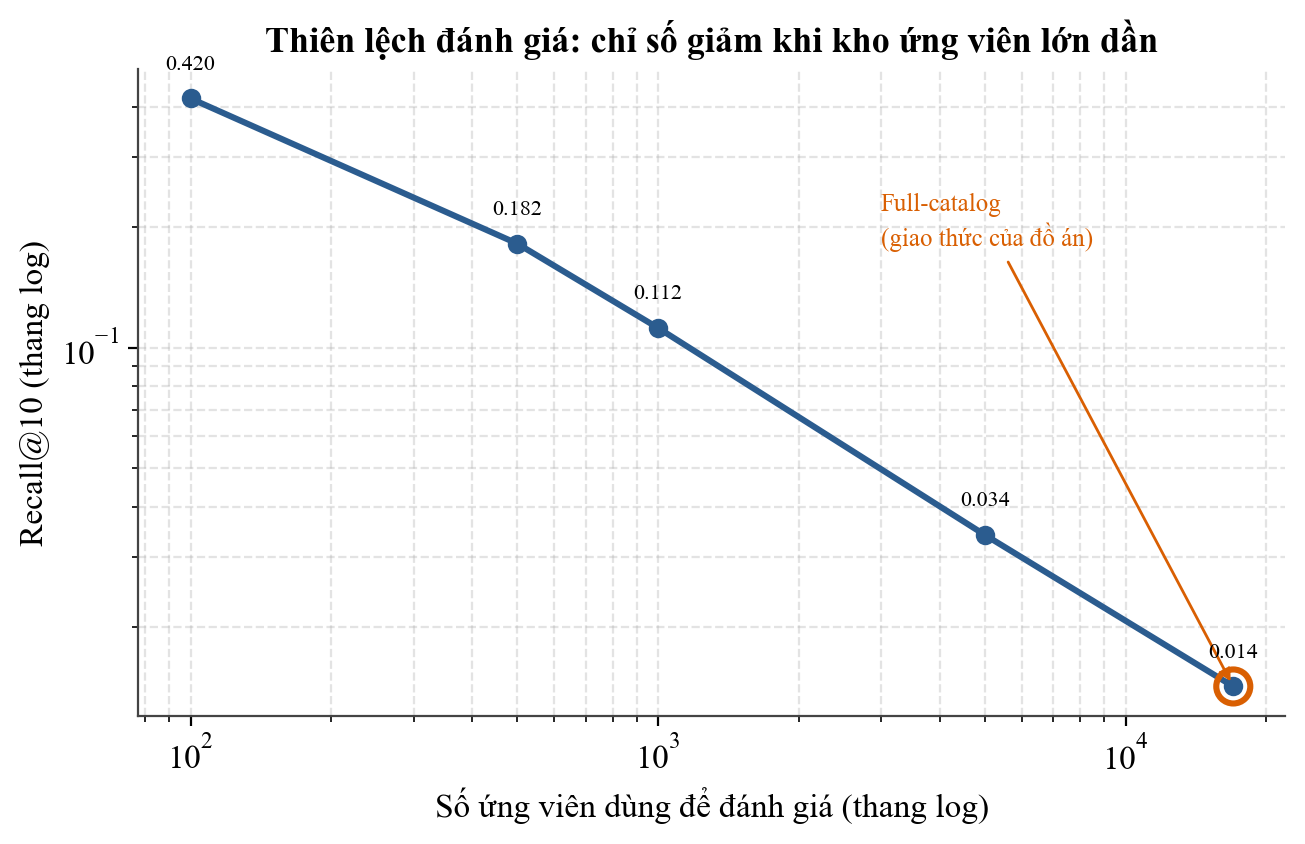
\includegraphics[width=0.72\textwidth]{eval_protocol.png}
\caption{Recall@10 giảm khi số ứng viên đánh giá tăng -- minh chứng thiên lệch lấy mẫu}
\label{fig:evalproto}
\end{figure}

% =====================================================================
%  CHƯƠNG 3: PHÂN TÍCH VÀ THIẾT KẾ HỆ THỐNG
% =====================================================================
\chapter{Phân tích và thiết kế hệ thống}
\label{chap:design}

\section{Kiến trúc tổng thể}

Hệ thống được thiết kế thành một pipeline gồm bốn giai đoạn nối tiếp, từ dữ liệu thô
tới danh sách gợi ý (Hình~\ref{fig:pipeline}): (1) tiền xử lý dữ liệu lớn bằng Spark
và lưu Parquet; (2) mã hóa "trải nghiệm" người dùng và tổng hợp lịch sử có trọng số
thời gian; (3) huấn luyện mô hình hai tháp với học tương phản; (4) đánh giá truy hồi
trên toàn bộ kho sản phẩm.

Hình~\ref{fig:pipeline} là sơ đồ khối chi tiết toàn bộ luồng -- từ dữ liệu thô, qua
xử lý dữ liệu lớn, trích xuất đặc trưng, tới mô hình và đánh giá -- kèm các tệp/đối
tượng trung gian (Parquet, vector lịch sử) chuyển giao giữa các giai đoạn.

\begin{figure}[H]
\centering
\begin{tikzpicture}[
    font=\scriptsize,
    io/.style={rectangle, rounded corners=2pt, draw=gray!55, fill=gray!12,
        line width=0.6pt, text width=2.0cm, minimum height=0.65cm, align=center},
    proc/.style={rectangle, rounded corners=2pt, draw=blue!55, fill=blue!12,
        line width=0.7pt, text width=6.6cm, minimum height=0.62cm, align=center},
    art/.style={rectangle, rounded corners=2pt, draw=violet!60, fill=violet!8,
        line width=0.7pt, text width=6.6cm, minimum height=0.55cm, align=center},
    mdl/.style={rectangle, rounded corners=2pt, draw=teal!60, fill=teal!10,
        line width=0.7pt, text width=3.0cm, minimum height=0.78cm, align=center},
    a/.style={-{Stealth[length=1.8mm]}, line width=0.7pt, gray!65},
    plab/.style={font=\scriptsize\bfseries, anchor=west}
]
% ===== GIAI ĐOẠN 1: XỬ LÝ DỮ LIỆU =====
\node[io] (rev)   at (-2.6,0) {Reviews\\(JSONL)};
\node[io] (meta)  at (0,0)    {Metadata\\(JSONL)};
\node[io] (split) at (2.6,0)  {Split CSV\\train/val/test};
\node[proc] (spark) at (0,-1.25) {\textbf{Apache Spark:} khử trùng lặp $\cdot$ broadcast join $\cdot$ dựng \texttt{semantic\_text} $\cdot$ \texttt{log1p}};
\node[art]  (parq)  at (0,-2.35) {\textbf{Parquet:} train / val / test \;+\; item};
\draw[a] (rev)--(spark); \draw[a] (meta)--(spark); \draw[a] (split)--(spark);
\draw[a] (spark)--(parq);
% ===== GIAI ĐOẠN 2: TRÍCH XUẤT ĐẶC TRƯNG =====
\node[proc, draw=orange!65, fill=orange!12] (enc) at (0,-4.25)
    {\textbf{Mã hóa trải nghiệm} bằng MiniLM (đóng băng) + mean pooling};
\node[proc, draw=orange!65, fill=orange!12] (agg) at (0,-5.35)
    {\textbf{Tổng hợp trọng số thời gian} (recency $\times$ rating)};
\node[art] (uvec) at (0,-6.45) {\textbf{Vector lịch sử người dùng} (384-d)};
\draw[a] (parq)--(enc); \draw[a] (enc)--(agg); \draw[a] (agg)--(uvec);
% ===== GIAI ĐOẠN 3: MÔ HÌNH =====
\node[mdl] (ut) at (-2.4,-8.7) {Tháp User\\(MLP $384{\to}512{\to}384$)};
\node[mdl, draw=gray!55, fill=gray!12] (it) at (2.4,-8.7) {Tháp Item\\(MiniLM, đóng băng)};
\node[mdl, draw=orange!70, fill=orange!14] (loss) at (0,-10.1) {Cosine + InfoNCE\\(in-batch negatives)};
\draw[a] (uvec)--(ut);
\draw[a, gray!55] (parq.east) to[out=0,in=90] (it.north);  % van ban item tu Parquet item
\draw[a] (ut)--(loss); \draw[a, gray!55] (it)--(loss);
\draw[a, dashed, orange!70] (loss.west) to[out=180,in=-90] node[left, font=\tiny] {cập nhật} (ut.south);
% ===== GIAI ĐOẠN 4: ĐÁNH GIÁ =====
\node[mdl, draw=teal!60, fill=teal!12] (metric) at (0,-12.3)
    {\textbf{Đánh giá full-catalog} ($\sim$17K item): Recall@K, NDCG@K};
\draw[a, teal!60] (loss)--(metric);
% ===== BĂNG NỀN CÁC GIAI ĐOẠN =====
\begin{scope}[on background layer]
\node[draw=blue!50, rounded corners=4pt, fill=blue!4, line width=0.8pt,
      fit=(rev)(split)(parq), inner sep=6pt] (b1) {};
\node[draw=orange!55, rounded corners=4pt, fill=orange!4, line width=0.8pt,
      fit=(enc)(uvec), inner sep=6pt] (b2) {};
\node[draw=teal!55, rounded corners=4pt, fill=teal!4, line width=0.8pt,
      fit=(ut)(it)(loss), inner sep=6pt] (b3) {};
\node[draw=teal!60, rounded corners=4pt, fill=teal!7, line width=0.8pt,
      fit=(metric), inner sep=5pt] (b4) {};
\end{scope}
\node[plab, blue!55!black]   at ([yshift=8pt]b1.north west) {1. XỬ LÝ DỮ LIỆU (Spark)};
\node[plab, orange!60!black] at ([yshift=8pt]b2.north west) {2. TRÍCH XUẤT ĐẶC TRƯNG};
\node[plab, teal!55!black]   at ([yshift=8pt]b3.north west) {3. MÔ HÌNH TWO-TOWER};
\node[plab, teal!55!black]   at ([yshift=7pt]b4.north west) {4. ĐÁNH GIÁ};
\end{tikzpicture}
\caption{Sơ đồ khối end-to-end: từ xử lý dữ liệu đến mô hình và đánh giá}
\label{fig:pipeline}
\end{figure}

\section{Dữ liệu và tiền xử lý bằng PySpark}

Dữ liệu sử dụng là \textbf{Amazon Reviews 2023} (nhóm McAuley Lab, UCSD), danh mục
\textit{Software}, gồm hai phần: tập \textbf{tương tác} (review của người dùng, các
trường \texttt{user\_id}, \texttt{parent\_asin}, \texttt{rating}, \texttt{title},
\texttt{text}, \texttt{timestamp}) và tập \textbf{metadata sản phẩm} (tiêu đề, tính
năng, mô tả, danh mục, giá, điểm trung bình\ldots). Quy mô bài toán được tổng hợp
trong Bảng~\ref{tab:stats}.

\begin{table}[H]
\centering
\caption{Thống kê quy mô bộ dữ liệu Amazon Software}
\label{tab:stats}
\renewcommand{\arraystretch}{1.3}
\begin{tabularx}{0.86\textwidth}{@{}X r@{}}
\toprule
\textbf{Thuộc tính} & \textbf{Giá trị} \\
\midrule
Số người dùng                         & $146.396$ \\
Số sản phẩm phần mềm độc nhất          & $> 17.000$ \\
Số tương tác huấn luyện (train)        & $\approx 984.000$ \\
Số mẫu kiểm định (validation)          & $146.396$ (1 / người dùng) \\
Số mẫu kiểm thử (test)                 & $146.396$ (1 / người dùng) \\
Số chiều vector biểu diễn              & $384$ \\
Thang điểm đánh giá                    & $1$ -- $5$ sao \\
\bottomrule
\end{tabularx}
\end{table}

Theo giao thức leave-last-out, mỗi người dùng đóng góp đúng một mẫu cho tập kiểm
định và một mẫu cho tập kiểm thử, phần còn lại thuộc tập huấn luyện. Phân phối số
tương tác trên mỗi người dùng (Hình~\ref{fig:userint}) lệch phải mạnh -- đa số người
dùng chỉ có vài tương tác, một thiểu số rất tích cực -- phản ánh tính thưa thớt và
đuôi dài đặc trưng của dữ liệu thương mại điện tử.

\begin{figure}[H]
\centering
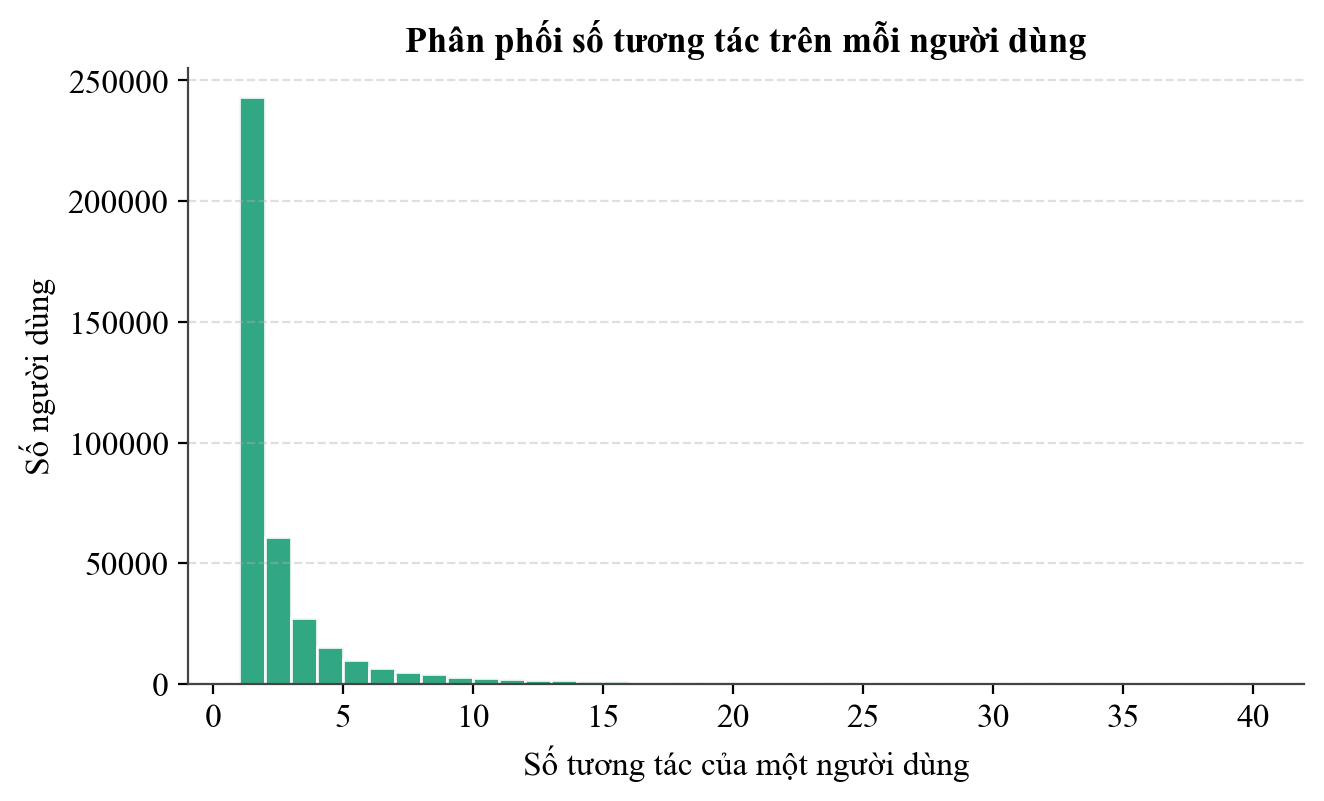
\includegraphics[width=0.72\textwidth]{user_interactions.png}
\caption{Phân phối số tương tác trên mỗi người dùng}
\label{fig:userint}
\end{figure}

\subsection{Làm sạch và kiểm tra chất lượng dữ liệu}

Dữ liệu thô từ Amazon chứa nhiều giá trị thiếu và bản ghi trùng. Quy trình làm sạch
trên Spark gồm: (i) \textbf{khai báo lược đồ tường minh} (\texttt{StructType}) khi
đọc metadata để kiểm soát kiểu dữ liệu của các trường phức tạp (mảng, map); (ii)
\textbf{đếm giá trị thiếu} từng cột để đánh giá chất lượng; (iii) \textbf{khử trùng
lặp} bằng \texttt{dropDuplicates}; và (iv) \textbf{ghép nối} tập chia chuẩn với dữ
liệu đầy đủ bằng \texttt{broadcast join} -- kỹ thuật phát tán bảng nhỏ tới mọi
executor, tránh thao tác shuffle tốn kém trên bảng lớn.

\begin{lstlisting}[language=Python, caption=Kiểm tra null và ghép nối broadcast trên Spark]
from pyspark.sql.functions import col, count, when, isnan, broadcast

# Dem so gia tri thieu tren tung cot
df.select([
    count(when(col(c).isNull(), c)).alias(c) for c in df.columns
]).show()

# Khu trung lap
df = df.dropDuplicates()

# Ghep tap split chuan (nho) voi du lieu day du (lon) bang broadcast join
df_train_ok = broadcast(df_train).join(
    df, on=["user_id", "parent_asin", "timestamp"], how="left")
\end{lstlisting}

Các trường số như \texttt{price} và \texttt{rating\_number} có phân phối lệch phải
rất mạnh nên được biến đổi \texttt{log1p} để nén khoảng giá trị, giúp ổn định khi
đưa vào mô hình. Cuối cùng, tập tương tác được lọc để chỉ giữ lại các sản phẩm tồn
tại trong bảng metadata, bảo đảm mọi sản phẩm đều có văn bản ngữ nghĩa.

\subsection{Dựng văn bản ngữ nghĩa cho sản phẩm}

Bước quan trọng nhất của tiền xử lý là tổng hợp các trường metadata rời rạc thành một
chuỗi văn bản ngữ nghĩa thống nhất (\texttt{semantic\_text}) để làm đầu vào cho mô
hình ngôn ngữ. Các trường dạng mảng được ghép bằng \texttt{concat\_ws}, trường
\texttt{details} dạng map được duyệt thành các dòng "khóa: giá trị":

\begin{lstlisting}[language=Python, caption=Dựng semantic\_text từ metadata bằng PySpark]
from pyspark.sql import functions as F

# Ghep cac truong mang (features, description, categories) thanh text
for c in ["features", "description", "categories"]:
    df_i = df_i.withColumn(f"{c}_text",
        F.when(F.col(c).isNotNull(), F.concat_ws(" ", F.col(c))).otherwise(F.lit("")))

# Tong hop semantic_text co cau truc theo tung khoi
df_i = df_i.withColumn("semantic_text", F.concat_ws("\n\n",
    F.when(F.col("title") != "",         F.concat(F.lit("TITLE\n"), F.col("title"))),
    F.when(F.col("features_text") != "", F.concat(F.lit("FEATURES\n"), F.col("features_text"))),
    F.when(F.col("description_text") != "", F.concat(F.lit("DESCRIPTION\n"), F.col("description_text"))),
    F.when(F.col("categories_text") != "", F.concat(F.lit("CATEGORIES\n"), F.col("categories_text")))))

# Chuan hoa truong so: log1p cho gia va so luong danh gia (giam lech phai)
df_i = df_i.withColumn("price", F.log1p(F.col("price")))
df_i = df_i.withColumn("rating_number", F.log1p(F.col("rating_number")))
\end{lstlisting}

Một ví dụ \texttt{semantic\_text} sau khi tổng hợp có dạng như sau:

\begin{lstlisting}[caption=Ví dụ văn bản ngữ nghĩa của một sản phẩm phần mềm]
TITLE
Norton 360 Deluxe 2024, Antivirus software for 5 Devices

FEATURES
Real-time protection against malware, ransomware and phishing
Secure VPN for online privacy; 50 GB cloud backup

CATEGORIES
Software | Antivirus & Security | Internet Security Suites
\end{lstlisting}

Khi đưa vào mô hình ngôn ngữ, toàn bộ khối văn bản này được nén thành một vector
$384$ chiều duy nhất, "hiểu" được rằng đây là phần mềm bảo mật -- nhờ đó các sản
phẩm cùng loại sẽ nằm gần nhau trong không gian biểu diễn.

Dữ liệu sau xử lý được lưu thành các tệp Parquet riêng cho tập huấn luyện, kiểm định,
kiểm thử và bảng sản phẩm. Phân phối điểm đánh giá (Hình~\ref{fig:rating}) lệch mạnh
về phía điểm cao -- đặc trưng điển hình của dữ liệu thương mại điện tử. Độ dài
\texttt{semantic\_text} (Hình~\ref{fig:textlen}) có trung vị khoảng $70$--$80$ token;
mô hình giới hạn \texttt{max\_length = 128} để cân bằng giữa thông tin và tốc độ.

\begin{figure}[H]
\centering
\begin{subfigure}{0.49\textwidth}
    \centering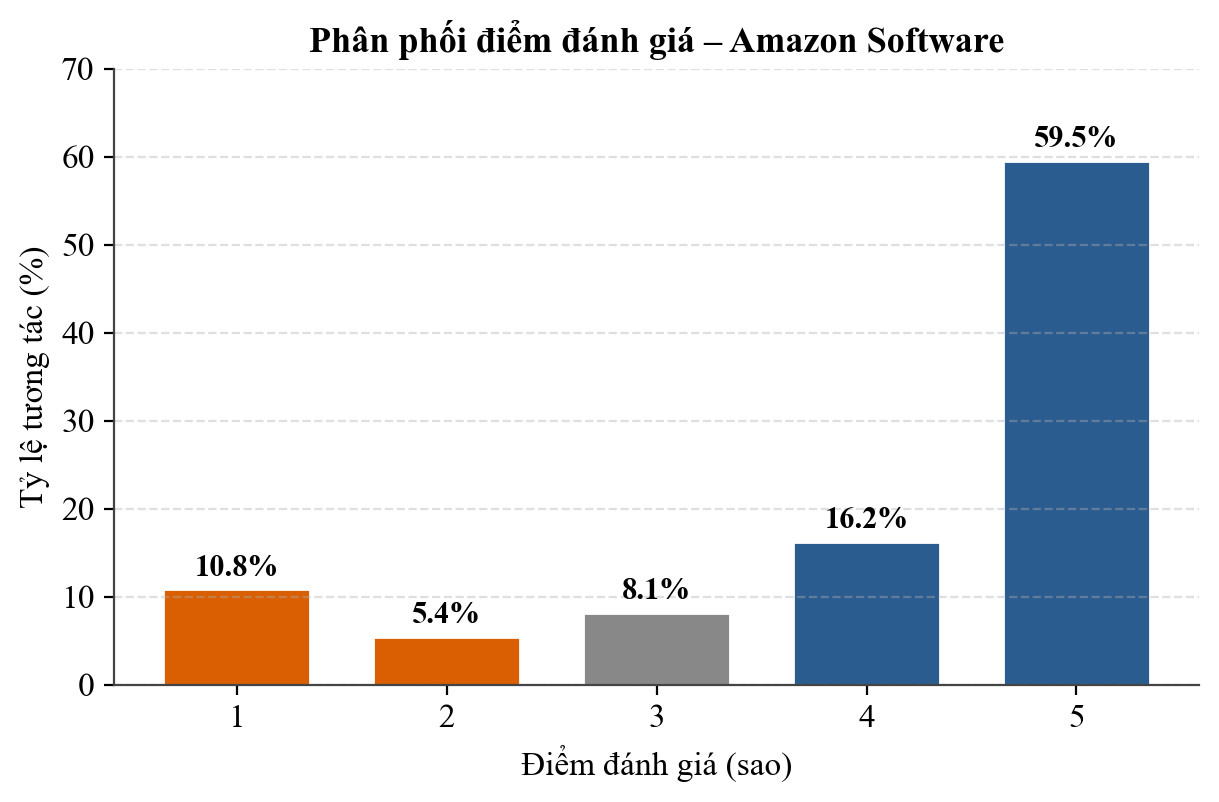
\includegraphics[width=\textwidth]{rating_distribution.png}
    \caption{Phân phối điểm đánh giá}
    \label{fig:rating}
\end{subfigure}
\hfill
\begin{subfigure}{0.49\textwidth}
    \centering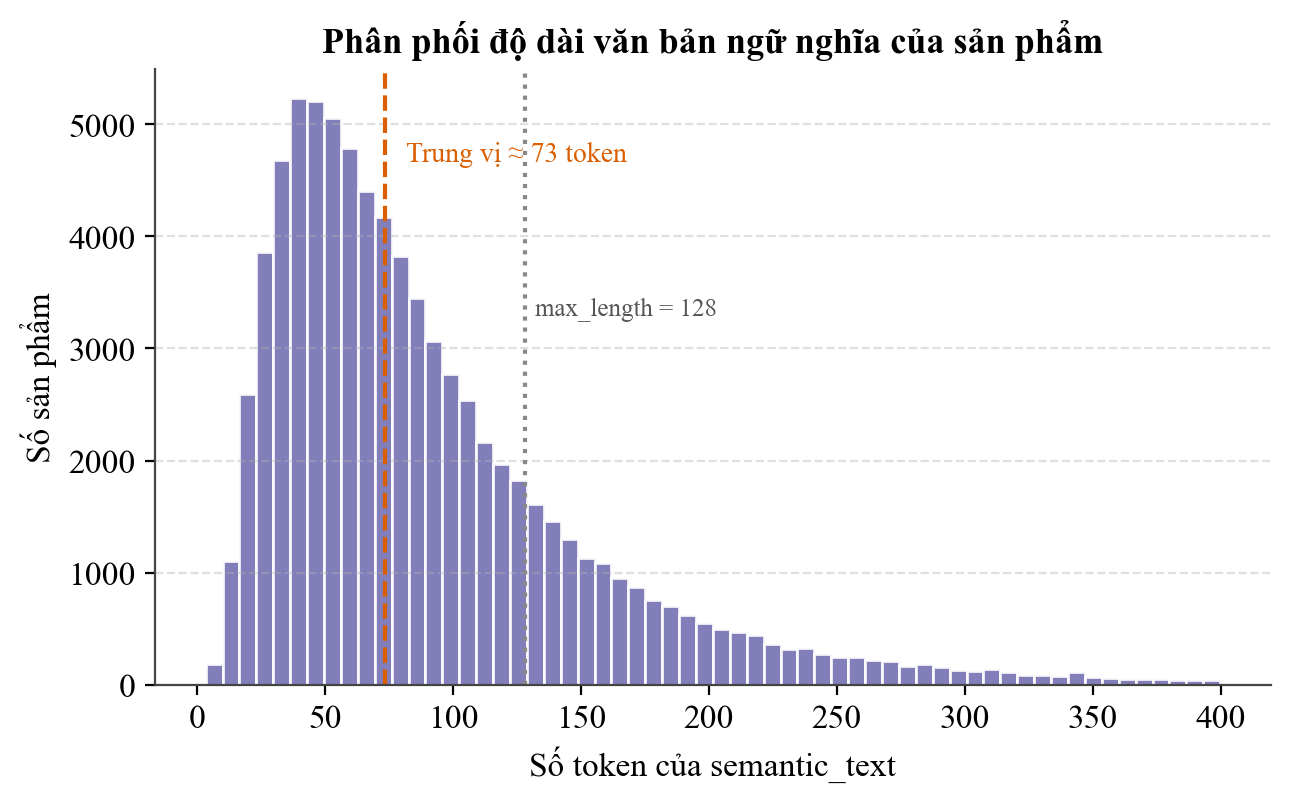
\includegraphics[width=\textwidth]{text_length.png}
    \caption{Độ dài semantic\_text}
    \label{fig:textlen}
\end{subfigure}
\caption{Một số đặc trưng của dữ liệu Amazon Software}
\label{fig:data-eda}
\end{figure}

\section{Chiến lược chia dữ liệu theo thời gian}

Để mô phỏng sát kịch bản thực tế (dự đoán hành vi \textit{tương lai} từ
\textit{quá khứ}), đồ án áp dụng phương pháp \textbf{cắt chuỗi hành vi theo thời
gian} (leave-last-out) cho mỗi người dùng:

\begin{itemize}[leftmargin=2em, itemsep=2pt]
    \item \textbf{Tập kiểm thử (test):} sản phẩm được tương tác \textit{cuối cùng}.
    \item \textbf{Tập kiểm định (validation):} sản phẩm \textit{kề cuối}.
    \item \textbf{Tập huấn luyện (train):} toàn bộ các tương tác \textit{trước đó}.
\end{itemize}

Cách chia này nghiêm ngặt hơn chia ngẫu nhiên vì tuyệt đối không để lộ thông tin
tương lai vào quá khứ (Hình~\ref{fig:loo}). Lịch sử của tập kiểm định kế thừa từ tập
huấn luyện; lịch sử của tập kiểm thử được tính trên hợp của tập huấn luyện và kiểm
định.

\begin{figure}[H]
\centering
\begin{tikzpicture}[font=\footnotesize,
    tr/.style={rectangle, rounded corners=2pt, draw=blue!55, fill=blue!10, minimum width=1.15cm, minimum height=0.8cm},
    va/.style={rectangle, rounded corners=2pt, draw=orange!70, fill=orange!15, minimum width=1.15cm, minimum height=0.8cm},
    te/.style={rectangle, rounded corners=2pt, draw=red!65, fill=red!12, minimum width=1.15cm, minimum height=0.8cm}]
\node[tr] (t1) {$i_1$};
\node[tr, right=0.18cm of t1] (t2) {$i_2$};
\node[right=0.18cm of t2] (dots) {$\cdots$};
\node[tr, right=0.18cm of dots] (t3) {$i_{n-2}$};
\node[va, right=0.18cm of t3] (t4) {$i_{n-1}$};
\node[te, right=0.18cm of t4] (t5) {$i_{n}$};
\draw[-{Stealth[length=2.4mm]}, line width=0.8pt, gray!70]
    ([yshift=-0.65cm]t1.south west) -- ([yshift=-0.65cm]t5.south east)
    node[midway, below, font=\scriptsize] {Thời gian};
\node[below=0.02cm of t1, font=\scriptsize, blue!55!black] {};
\draw[decorate, decoration={brace, amplitude=4pt}, blue!55]
    (t1.north west) -- (t3.north east) node[midway, above=3pt, font=\scriptsize\bfseries, blue!55!black] {Train};
\node[above=0.5cm of t4, font=\scriptsize\bfseries, orange!70!black] {Val};
\node[above=0.5cm of t5, font=\scriptsize\bfseries, red!65!black] {Test};
\draw[-{Stealth[length=1.6mm]}, orange!70] ([yshift=0.32cm]t4.north) -- (t4.north);
\draw[-{Stealth[length=1.6mm]}, red!65] ([yshift=0.32cm]t5.north) -- (t5.north);
\end{tikzpicture}
\caption{Chia dữ liệu leave-last-out: mục cuối làm test, kề cuối làm val, còn lại train}
\label{fig:loo}
\end{figure}

\section{Mã hóa trải nghiệm và tổng hợp lịch sử người dùng}

\subsection{Mã hóa trải nghiệm}

Trước hết, mỗi sản phẩm được biểu diễn bằng một chuỗi văn bản tổng hợp
(\texttt{item\_text\_map}) ghép \texttt{semantic\_text} với các thuộc tính bổ sung
(danh mục, cửa hàng, giá, điểm và số lượng đánh giá):

\begin{lstlisting}[language=Python, caption=Dựng từ điển văn bản sản phẩm item\_text\_map]
item_text_map = {}
for r in item_df.itertuples():
    item_text_map[r.parent_asin] = (
        f"{safe(r.semantic_text)}\n"
        f"Category: {safe(r.main_category)}\nStore: {safe(r.store)}\n"
        f"Price: {safe(r.price)}\nAverage Rating: {safe(r.average_rating)}\n"
        f"Rating Count: {safe(r.rating_number)}")
\end{lstlisting}

Mỗi tương tác của người dùng được biến thành một "trải nghiệm" bằng cách ghép văn bản
sản phẩm trên với tiêu đề và nội dung review, rồi mã hóa qua mô hình MiniLM (đóng băng)
theo từng batch trên GPU:

\begin{lstlisting}[language=Python, caption=Mã hóa trải nghiệm người dùng hàng loạt trên GPU]
def precompute_user_experience_vectors(df, batch_size=256):
    base = df['parent_asin'].map(item_text_map).fillna('None')
    combined = (base + "\nUser Review Title: " + df['title'].fillna('None')
                     + "\nUser Review Content: " + df['text'].fillna('None')).tolist()
    vectors = []
    with torch.no_grad():
        for i in range(0, len(combined), batch_size):
            enc = tokenizer(combined[i:i+batch_size], padding=True, truncation=True,
                            max_length=128, return_tensors="pt").to(device)
            out = base_model(**enc)
            emb = F.normalize(mean_pooling(out, enc["attention_mask"]), dim=1)
            vectors.append(emb.cpu().numpy())
    return np.vstack(vectors)
\end{lstlisting}

\subsection{Tổng hợp lịch sử với trọng số thời gian}

Vector đại diện cho một người dùng là \textit{trung bình có trọng số} của các vector
trải nghiệm trong lịch sử. Trọng số kết hợp hai yếu tố: (i) \textbf{độ gần đây}
(recency) -- tương tác càng mới càng quan trọng, theo hàm suy giảm mũ
$e^{-(n-i)/n}$; và (ii) \textbf{mức độ ưa thích} -- điểm rating càng cao trọng số
càng lớn, theo hệ số $(1 + \text{rating}/5)$:

\begin{equation}
    \mathbf{u} = \frac{\sum_{i=1}^{n} w_i\, \mathbf{e}_i}{\sum_{i=1}^{n} w_i},
    \qquad
    w_i = e^{-(n-i)/n} \cdot \left(1 + \frac{\text{rating}_i}{5}\right),
\end{equation}

trong đó $\mathbf{e}_i$ là vector trải nghiệm thứ $i$ và $n$ là số tương tác của
người dùng. Vector kết quả được chuẩn hóa $L_2$. Hình~\ref{fig:timedecay} minh họa
cách trọng số tăng dần về phía các tương tác gần đây nhất. Toàn bộ phép tổng hợp này
chạy trên CPU/RAM (gom nhóm theo \texttt{user\_id}), độc lập với GPU, nên rất nhẹ và
nhanh.

\begin{lstlisting}[language=Python, caption=Tổng hợp vector lịch sử có trọng số thời gian]
def aggregate_user_history(df, experience_vectors):
    df['_vec'] = list(experience_vectors)
    user_hist = {}
    for uid, g in df.groupby("user_id"):
        g = g.reset_index(drop=True); n = len(g)
        vectors = np.array(g['_vec'].tolist())
        idx = np.arange(n)
        recency = np.exp(-(n - idx) / max(n, 1))          # cang moi cang nang
        ratings = g['rating'].fillna(0).to_numpy()
        weights = (recency * (1 + ratings / 5.0)).reshape(-1, 1)
        u = np.sum(vectors * weights, axis=0) / np.sum(weights)
        user_hist[uid] = u / (np.linalg.norm(u) + 1e-9)   # chuan hoa L2
    return user_hist
\end{lstlisting}

Phép \textbf{mean pooling có mặt nạ} (dùng ở cả khâu mã hóa) lấy trung bình các vector
token, bỏ qua token đệm nhờ \texttt{attention\_mask}:

\begin{lstlisting}[language=Python, caption=Mean pooling có mặt nạ]
def mean_pooling(out, mask):
    token = out.last_hidden_state                      # [B, L, 384]
    mask = mask.unsqueeze(-1).expand(token.size()).float()
    return (token * mask).sum(1) / torch.clamp(mask.sum(1), min=1e-9)
\end{lstlisting}

\begin{figure}[H]
\centering
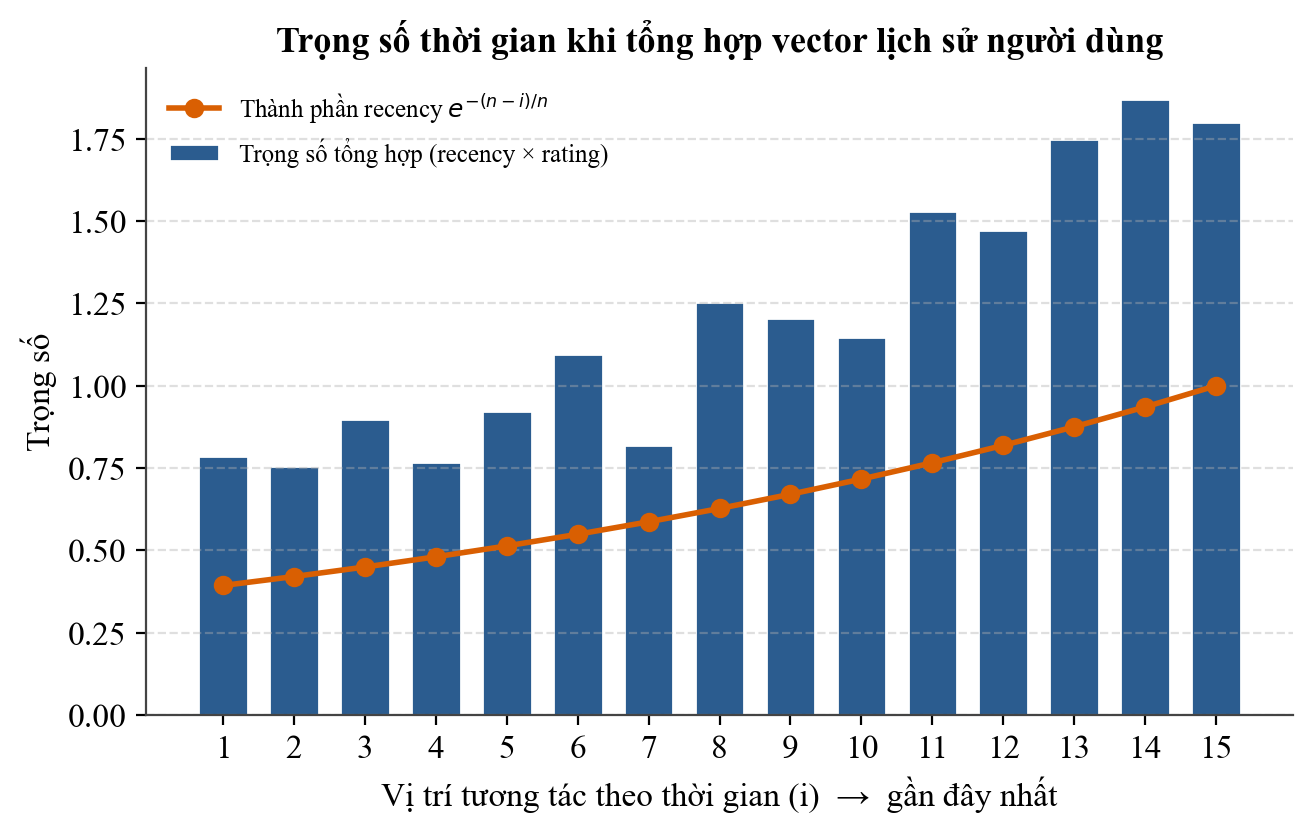
\includegraphics[width=0.74\textwidth]{time_decay.png}
\caption{Trọng số thời gian khi tổng hợp vector lịch sử người dùng ($n = 15$)}
\label{fig:timedecay}
\end{figure}

Toàn bộ luồng tổng hợp được tóm tắt trong Hình~\ref{fig:aggflow}: các vector trải
nghiệm được nhân với trọng số tương ứng, cộng lại rồi chuẩn hóa thành một vector
người dùng duy nhất.

\begin{figure}[H]
\centering
\begin{tikzpicture}[font=\footnotesize, node distance=0.7cm,
    e/.style={rectangle, rounded corners=2pt, draw=blue!55, fill=blue!9, minimum width=1.3cm, minimum height=0.7cm},
    op/.style={circle, draw=teal!60, fill=teal!12, minimum size=0.8cm},
    o/.style={rectangle, rounded corners=2pt, draw=orange!70, fill=orange!12, minimum width=1.8cm, minimum height=0.7cm},
    a/.style={-{Stealth[length=2mm]}, line width=0.7pt, blue!55}]
\node[e] (e1) {$\mathbf{e}_1$};
\node[e, below=0.3cm of e1] (e2) {$\mathbf{e}_2$};
\node[below=0.18cm of e2, font=\scriptsize] (ed) {$\vdots$};
\node[e, below=0.25cm of ed] (en) {$\mathbf{e}_n$};
\node[op, right=1.6cm of e2] (sum) {$\sum$};
\node[o, right=1.3cm of sum] (norm) {L2 Normalize};
\node[o, right=0.9cm of norm, fill=orange!18] (u) {$\mathbf{u}$};
\draw[a] (e1) -- node[above, font=\scriptsize, pos=0.45] {$\times w_1$} (sum);
\draw[a] (e2) -- node[above, font=\scriptsize, pos=0.5] {$\times w_2$} (sum);
\draw[a] (en) -- node[below, font=\scriptsize, pos=0.45] {$\times w_n$} (sum);
\draw[a] (sum) -- (norm);
\draw[a] (norm) -- (u);
\node[below=0.55cm of sum, font=\scriptsize, gray!55!black, text width=3cm, align=center]
    {$w_i = e^{-(n-i)/n}(1+\text{rating}_i/5)$};
\end{tikzpicture}
\caption{Luồng tổng hợp vector lịch sử người dùng từ các vector trải nghiệm}
\label{fig:aggflow}
\end{figure}

\section{Thiết kế mô hình hai tháp}

Mô hình \texttt{TwoTowerVectorModel} hiện thực hóa kiến trúc ở
Mục~\ref{sec:twotower}. \textbf{Tháp người dùng} là một mạng MLP biến đổi vector
lịch sử $384$ chiều, có \texttt{BatchNorm} để ổn định gradient và \texttt{Dropout}
để chống quá khớp. \textbf{Tháp sản phẩm} là MiniLM \textbf{đóng băng}, chỉ làm
nhiệm vụ mã hóa văn bản.

\begin{lstlisting}[language=Python, caption=Mô hình hai tháp (tháp sản phẩm đóng băng)]
class TwoTowerVectorModel(nn.Module):
    def __init__(self, model_name):
        super().__init__()
        # Thap User: MLP co the huan luyen
        self.user_projection = nn.Sequential(
            nn.Linear(384, 512), nn.BatchNorm1d(512), nn.ReLU(),
            nn.Dropout(0.5), nn.Linear(512, 384))
        # Thap Item: dong bang hoan toan
        self.item_encoder = AutoModel.from_pretrained(model_name)
        for p in self.item_encoder.parameters():
            p.requires_grad = False

    def forward_user(self, user_vectors):
        return F.normalize(self.user_projection(user_vectors), dim=1)

    def forward_item(self, tokens):
        with torch.no_grad():
            out = self.item_encoder(**tokens)
            emb = self.mean_pooling(out, tokens["attention_mask"])
        return F.normalize(emb, dim=1)
\end{lstlisting}

\subsection{Sơ đồ kiến trúc chi tiết}

Hình~\ref{fig:model-detail} mô tả chi tiết từng tầng của mô hình cùng kích thước
tensor tương ứng ($B$ là kích thước batch, $L$ là độ dài chuỗi token). Tháp người
dùng biến đổi vector lịch sử qua một khối MLP, còn tháp sản phẩm đưa chuỗi token qua
$6$ tầng Transformer của MiniLM rồi gộp trung bình. Hai vector đầu ra cùng kích
thước $384$ chiều được chuẩn hóa và đem so khớp bằng tích vô hướng.

\begin{figure}[H]
\centering
\begin{tikzpicture}[
    font=\scriptsize,
    layer/.style={rectangle, rounded corners=2pt, draw=blue!55, fill=blue!8,
        line width=0.7pt, text width=2.75cm, minimum height=0.6cm, align=center},
    frozen/.style={rectangle, rounded corners=2pt, draw=gray!60, fill=gray!12,
        line width=0.7pt, text width=2.75cm, minimum height=0.6cm, align=center},
    io/.style={rectangle, rounded corners=2pt, draw=teal!60, fill=teal!10,
        line width=0.7pt, text width=2.75cm, minimum height=0.6cm, align=center},
    sh/.style={font=\scriptsize\itshape, text=gray!55!black},
    a/.style={-{Stealth[length=1.6mm]}, line width=0.6pt, blue!55},
    ag/.style={-{Stealth[length=1.6mm]}, line width=0.6pt, gray!60}
]
% ===== USER TOWER (left) =====
\node[io] (uin) {Vector lịch sử người dùng};
\node[sh, right=0.15cm of uin] {[B, 384]};
\node[layer, above=0.4cm of uin] (l1) {Linear $384 \to 512$};
\node[sh, right=0.15cm of l1] {[B, 512]};
\node[layer, above=0.35cm of l1] (l2) {BatchNorm1d(512)};
\node[layer, above=0.35cm of l2] (l3) {ReLU};
\node[layer, above=0.35cm of l3] (l4) {Dropout($0.5$)};
\node[layer, above=0.35cm of l4] (l5) {Linear $512 \to 384$};
\node[sh, right=0.15cm of l5] {[B, 384]};
\node[io, above=0.4cm of l5] (un) {L2 Normalize};
\draw[a] (uin)--(l1); \draw[a] (l1)--(l2); \draw[a] (l2)--(l3);
\draw[a] (l3)--(l4); \draw[a] (l4)--(l5); \draw[a] (l5)--(un);

% ===== ITEM TOWER (right) =====
\node[io, right=3.0cm of uin] (iin) {Tokens semantic\_text};
\node[sh, right=0.15cm of iin] {[B, L]};
\node[frozen, above=0.4cm of iin] (e1) {Embedding};
\node[sh, right=0.15cm of e1] {[B, L, 384]};
\node[frozen, above=0.35cm of e1] (e2) {Transformer $\times\,6$\\(self-attention + FFN)};
\node[sh, right=0.15cm of e2] {[B, L, 384]};
\node[frozen, above=0.62cm of e2] (e3) {Mean Pooling (có mặt nạ)};
\node[sh, right=0.15cm of e3] {[B, 384]};
\node[io, above=0.4cm of e3] (inr) {L2 Normalize};
\draw[ag] (iin)--(e1); \draw[ag] (e1)--(e2); \draw[ag] (e2)--(e3); \draw[ag] (e3)--(inr);
\node[font=\scriptsize\bfseries, below=0.12cm of iin, text=gray!55!black]
    {Tháp Item (đóng băng)};
\node[font=\scriptsize\bfseries, below=0.12cm of uin, text=blue!55!black]
    {Tháp User (huấn luyện)};

% ===== TOP: similarity =====
\node[rectangle, rounded corners=3pt, draw=orange!70, fill=orange!12,
      line width=0.9pt, text width=4.8cm, align=center, minimum height=0.75cm,
      above=1.15cm of $(un)!0.5!(inr)$] (sim)
      {Ma trận tương đồng $\mathbf{U}\mathbf{V}^\top$ $\;$[B, B]\\$\to$ InfoNCE Loss};
\draw[a] (un) |- (sim);
\draw[ag] (inr) |- (sim);
\end{tikzpicture}
\caption{Sơ đồ kiến trúc chi tiết của mô hình hai tháp kèm kích thước tensor}
\label{fig:model-detail}
\end{figure}

\subsection{Phân tích số tham số}

Một ưu điểm nổi bật của thiết kế là \textbf{hiệu quả tham số}. Bảng~\ref{tab:params}
liệt kê số tham số của tháp người dùng -- chỉ khoảng $395.000$ tham số khả huấn
luyện, trong khi tháp sản phẩm (MiniLM) có $\sim 22{,}7$ triệu tham số nhưng được
\textbf{đóng băng hoàn toàn}. Như vậy, chỉ khoảng \textbf{$1{,}7\%$} tổng số tham số
thực sự được cập nhật (Hình~\ref{fig:params}), giúp giảm mạnh chi phí bộ nhớ và thời
gian huấn luyện.

\begin{table}[H]
\centering
\caption{Số tham số khả huấn luyện của tháp người dùng}
\label{tab:params}
\renewcommand{\arraystretch}{1.25}
\begin{tabularx}{0.82\textwidth}{@{}X r@{}}
\toprule
\textbf{Tầng} & \textbf{Số tham số} \\
\midrule
Linear $384 \to 512$        & $197.120$ \\
BatchNorm1d$(512)$          & $1.024$ \\
Linear $512 \to 384$        & $196.992$ \\
\midrule
\textbf{Tổng (khả huấn luyện)} & $\mathbf{395.136}$ \\
Tháp Item (MiniLM, đóng băng)  & $\approx 22.700.000$ \\
\bottomrule
\end{tabularx}
\end{table}

\begin{figure}[H]
\centering
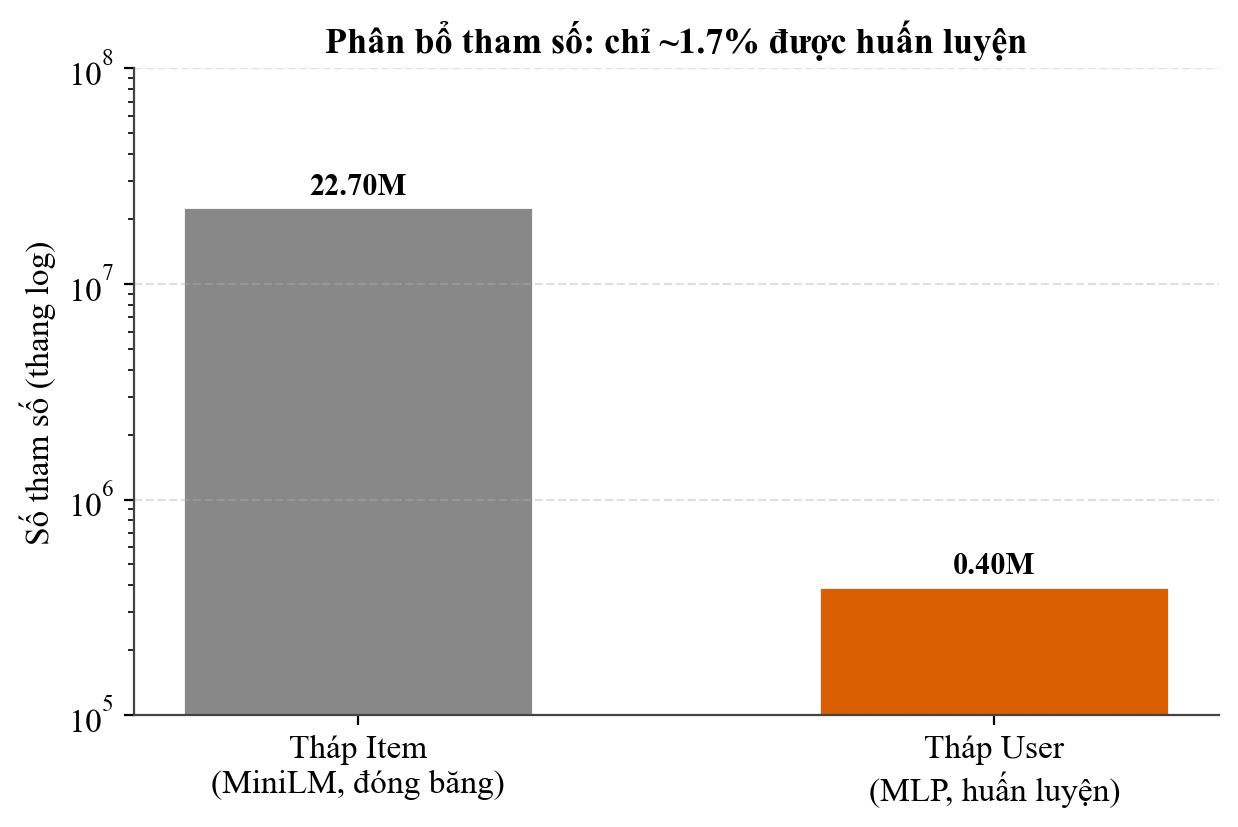
\includegraphics[width=0.62\textwidth]{param_breakdown.png}
\caption{Phân bổ tham số giữa hai tháp (chỉ $\sim 1{,}7\%$ được huấn luyện)}
\label{fig:params}
\end{figure}

\section{Hàm mất mát và cấu hình huấn luyện}

Mô hình được huấn luyện bằng hàm mất mát \textbf{InfoNCE} (Mục~\ref{sec:infonce})
với mẫu âm trong batch. Ma trận tương đồng giữa mọi người dùng và mọi sản phẩm trong
batch được tính, nhãn đúng nằm trên đường chéo:

\begin{lstlisting}[language=Python, caption=Hàm mất mát InfoNCE với mẫu âm trong batch]
class InfoNCE(nn.Module):
    def __init__(self, temperature=0.1):
        super().__init__()
        self.temperature = temperature
        self.ce = nn.CrossEntropyLoss()

    def forward(self, user_out, item_out):
        sim = torch.matmul(user_out, item_out.T) / self.temperature
        labels = torch.arange(user_out.size(0), device=user_out.device)
        return self.ce(sim, labels)

loss_fn = InfoNCE(temperature=0.1)
optimizer = torch.optim.AdamW(model.parameters(), lr=1e-4, weight_decay=5e-2)
\end{lstlisting}

Mô hình được tối ưu bằng \texttt{AdamW} (learning rate $10^{-4}$, weight decay
$0{,}05$). Quá trình huấn luyện áp dụng \textbf{tính toán độ chính xác hỗn hợp}
(mixed precision) để tiết kiệm bộ nhớ GPU và tăng tốc, kèm cơ chế dừng sớm (early
stopping) dựa trên mất mát kiểm định. Chi tiết cấu hình và kết quả được trình bày ở
Chương~\ref{chap:exp}.

% =====================================================================
%  CHƯƠNG 4: KẾT QUẢ THỰC NGHIỆM
% =====================================================================
\chapter{Kết quả thực nghiệm}
\label{chap:exp}

\section{Môi trường và cấu hình}

Toàn bộ thực nghiệm được triển khai trên môi trường điện toán đám mây
\textbf{Google Colab} với bộ xử lý đồ họa (GPU) gia tốc. Để tối ưu vùng nhớ và tốc
độ, đồ án sử dụng kỹ thuật \textbf{tính toán độ chính xác hỗn hợp} (mixed precision)
thông qua \texttt{torch.amp} kết hợp \texttt{GradScaler}. Bảng~\ref{tab:hyper} tổng
hợp các siêu tham số chính.

\begin{table}[H]
\centering
\caption{Cấu hình môi trường và siêu tham số huấn luyện}
\label{tab:hyper}
\renewcommand{\arraystretch}{1.3}
\begin{tabularx}{\textwidth}{@{}l X@{}}
\toprule
\textbf{Thành phần} & \textbf{Cấu hình} \\
\midrule
Bộ mã hóa văn bản (tháp Item) & \texttt{all-MiniLM-L6-v2} ($6$ tầng, $384$ chiều), đóng băng \\
Tháp người dùng & MLP $384{\to}512{\to}384$, BatchNorm, ReLU, Dropout $0{,}5$ \\
Hàm mất mát & InfoNCE (in-batch negatives), temperature $\tau = 0{,}1$ \\
Bộ tối ưu & AdamW, learning rate $10^{-4}$, weight decay $0{,}05$ \\
Batch size & $256$ \\
Số epoch & $5$ (early stopping theo val loss) \\
Độ chính xác & Mixed precision (FP16) trên GPU \\
Nạp dữ liệu & Parquet + DataLoader $2$ worker, bất đồng bộ \\
\bottomrule
\end{tabularx}
\end{table}

Quy mô dữ liệu: khoảng $984.000$ tương tác huấn luyện ($3.844$ batch mỗi epoch),
$146.396$ người dùng và hơn $17.000$ sản phẩm. Bảng~\ref{tab:time} phân rã thời gian
một epoch: phần lớn dành cho huấn luyện ($\sim 38$ phút), phần còn lại cho tính mất
mát kiểm định và đánh giá toàn kho ($\sim 11$ phút).

\begin{table}[H]
\centering
\caption{Phân rã thời gian một epoch (tốc độ $\sim 1{,}7$ batch/giây)}
\label{tab:time}
\renewcommand{\arraystretch}{1.25}
\begin{tabularx}{0.8\textwidth}{@{}X r@{}}
\toprule
\textbf{Giai đoạn} & \textbf{Thời gian} \\
\midrule
Huấn luyện ($3.844$ batch)            & $\approx 38$ phút \\
Tính mất mát kiểm định ($572$ batch)  & $\approx 5{,}7$ phút \\
Mã hóa kho item + tính Recall/NDCG    & $\approx 5{,}4$ phút \\
\midrule
\textbf{Tổng mỗi epoch}               & $\approx 49$ phút \\
\bottomrule
\end{tabularx}
\end{table}

\section{Chi tiết vòng lặp huấn luyện}

Vòng lặp huấn luyện kết hợp nhiều kỹ thuật để tối ưu tốc độ và bộ nhớ. Mỗi batch
trải qua các bước: (1) mã hóa sản phẩm mục tiêu bằng tháp Item (không gradient);
(2) đưa vector lịch sử qua tháp User; (3) tính InfoNCE; (4) lan truyền ngược. Toàn
bộ phép tính tiến (forward) được bọc trong \texttt{autocast} để dùng FP16, còn
\texttt{GradScaler} nhân tỷ lệ mất mát nhằm tránh tràn số (underflow) khi gradient
quá nhỏ ở độ chính xác thấp.

\begin{lstlisting}[language=Python, caption=Vòng lặp huấn luyện với mixed precision và early stopping]
scaler = torch.amp.GradScaler('cuda')
best_val_loss = float('inf'); patience_counter = 0

for epoch in range(EPOCHS):
    model.train(); total_loss = 0
    for batch in train_loader:
        item_tokens = {k: v.to(device) for k, v in batch["item_tokens"].items()}
        optimizer.zero_grad()
        with torch.amp.autocast('cuda'):          # mixed precision FP16
            item_out = model.forward_item(item_tokens)        # thap dong bang
            user_out = model.forward_user(batch["user_vectors"].to(device))
            loss = loss_fn(user_out, item_out)                # InfoNCE
        scaler.scale(loss).backward()              # scale tranh underflow
        scaler.step(optimizer); scaler.update()
        total_loss += loss.item()

    val_loss = compute_loss(model, val_loader, loss_fn, device)
    if val_loss < best_val_loss:                   # early stopping theo val loss
        best_val_loss = val_loss; patience_counter = 0
        torch.save(model.state_dict(), best_model_path)
    else:
        patience_counter += 1
        if patience_counter >= PATIENCE: break
\end{lstlisting}

Cơ chế \textbf{early stopping} lưu lại trọng số tốt nhất mỗi khi mất mát kiểm định
giảm và dừng huấn luyện nếu không cải thiện sau \texttt{PATIENCE} epoch -- bảo đảm
mô hình cuối cùng là phiên bản tổng quát hóa tốt nhất, tránh lãng phí tính toán.

\section{Thiết kế nạp dữ liệu theo batch}

Việc nạp dữ liệu được tổ chức qua lớp \texttt{Dataset} trả về vector người dùng (đã
tính sẵn) cùng văn bản sản phẩm mục tiêu, và một hàm \texttt{collate} gom batch:
chỉ \textit{văn bản sản phẩm} mới cần tokenize tại thời điểm tạo batch, còn vector
người dùng đã được mã hóa trước nên chỉ việc xếp chồng -- giảm đáng kể khối lượng
tính toán lặp lại. \texttt{DataLoader} dùng $2$ worker và \texttt{pin\_memory} để
nạp bất đồng bộ, che giấu độ trễ I/O sau thời gian tính toán của GPU.

\begin{lstlisting}[language=Python, caption=Hàm collate chỉ tokenize nhánh sản phẩm]
def collate_vector_fn(batch):
    user_vectors = torch.stack([b["user_vector"] for b in batch])  # [B, 384]
    item_texts = [b["item_text"] for b in batch]
    item_tokens = tokenizer(item_texts, padding=True, truncation=True,
                            max_length=128, return_tensors="pt")
    return {"user_vectors": user_vectors, "item_tokens": item_tokens,
            "target": [b["target"] for b in batch]}
\end{lstlisting}

\section{Giao thức đánh giá toàn kho (Full-catalog)}

Một đóng góp quan trọng về mặt phương pháp là cách đánh giá. Nhiều nghiên cứu chỉ
đánh giá trên một nhóm nhỏ mẫu âm lấy ngẫu nhiên (in-batch / sampled metrics), dẫn
tới chỉ số bị \textit{thổi phồng} và không phản ánh độ khó thực tế. Đồ án triệt tiêu
hoàn toàn thiên lệch này bằng giao thức \textbf{full-catalog}:

\begin{enumerate}[leftmargin=2em, itemsep=2pt]
    \item Mã hóa trước \textbf{toàn bộ} hơn $17.000$ sản phẩm thành ma trận vector
    sản phẩm.
    \item Với mỗi người dùng, tính độ tương đồng với \textit{tất cả} sản phẩm trong
    kho, lấy Top-$50$.
    \item Đo Recall@K và NDCG@K bằng cách kiểm tra sản phẩm mục tiêu thật có nằm
    trong Top-$K$ hay không.
\end{enumerate}

Việc tính toán được chia theo cụm người dùng ($1.000$ người mỗi lần) để tránh tràn
bộ nhớ GPU. Đây là cách đánh giá \textit{khắt khe và trung thực} nhất, vì người dùng
phải cạnh tranh với toàn bộ kho sản phẩm.

Về mặt kỹ thuật, nếu nhân trực tiếp ma trận người dùng ($146.396 \times 384$) với
ma trận sản phẩm ($17.000 \times 384$) sẽ tạo ra ma trận điểm số khổng lồ vượt quá
VRAM. Giải pháp là \textbf{xử lý theo cụm}: kho sản phẩm được mã hóa trước thành một
ma trận cố định; sau đó với mỗi cụm $1.000$ người dùng, ta tính điểm số, lấy
\texttt{topk} rồi giải phóng bộ nhớ trước khi sang cụm tiếp theo.

\begin{lstlisting}[language=Python, caption=Đánh giá toàn kho theo cụm để tránh tràn VRAM]
# Ma hoa truoc TOAN BO kho item mot lan
all_item_emb = encode_all_items(item_ids, model)        # [N_items, 384]

for i in range(0, num_users, 1000):                      # xu ly 1000 user/lan
    user_chunk = all_user_emb[i:i+1000].to(device)
    scores = torch.matmul(user_chunk, all_item_emb.T)    # [1000, N_items]
    _, topk = torch.topk(scores, k=50, dim=1)            # lay Top-50
    hits = (topk == target_chunk.view(-1, 1))            # vi tri trung
    recall10 += hits[:, :10].any(dim=1).float().sum().item()
    # ... cong don NDCG theo thu hang ...
    del scores, topk; torch.cuda.empty_cache()           # giai phong VRAM
\end{lstlisting}

Nhờ chiến lược này, hệ thống có thể đánh giá trên toàn bộ $146.396$ người dùng $\times$
$17.000$ sản phẩm mà vẫn nằm trong giới hạn bộ nhớ của một GPU phổ thông.

\section{Kết quả huấn luyện}

Hình~\ref{fig:loss} thể hiện đường cong mất mát qua $5$ epoch. Mất mát huấn luyện
(InfoNCE) giảm rõ từ $3{,}62$ xuống $3{,}31$, trong khi mất mát kiểm định
\textit{giảm đều đặn} từ $5{,}19$ xuống $5{,}16$ -- cho thấy mô hình hội tụ ổn định
và \textbf{không bị quá khớp}. Cơ chế early stopping lưu lại mô hình tốt nhất tại
mỗi lần val loss giảm; mô hình đạt trạng thái ổn định tại epoch thứ $5$.

\begin{figure}[H]
\centering
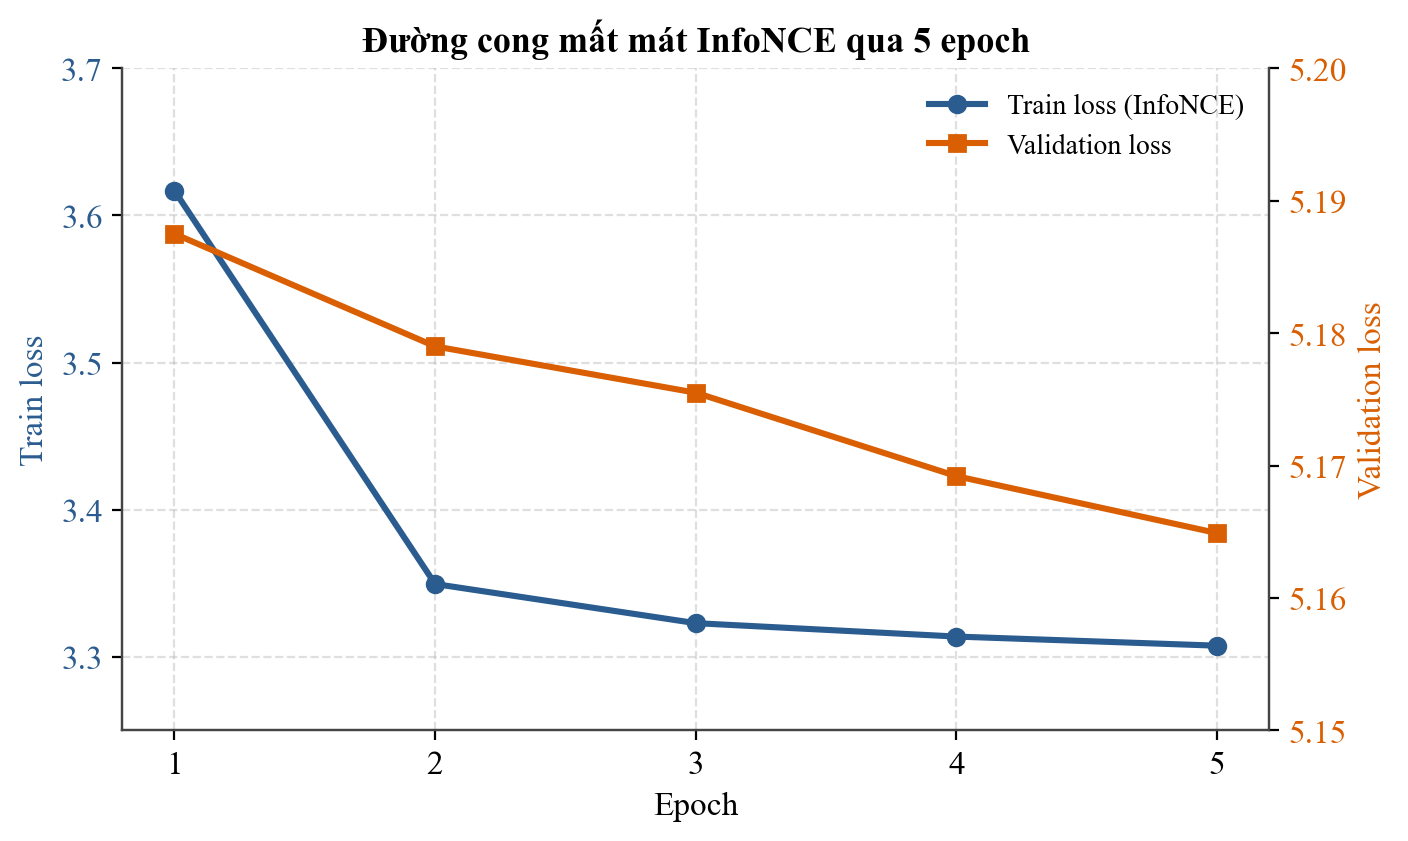
\includegraphics[width=0.78\textwidth]{loss_curve.png}
\caption{Đường cong mất mát InfoNCE trên tập huấn luyện và kiểm định}
\label{fig:loss}
\end{figure}

\section{Kết quả truy hồi trên toàn kho}

Bảng~\ref{tab:results} trình bày kết quả Recall@K và NDCG@K theo từng epoch trên tập
kiểm định, trực quan hóa ở Hình~\ref{fig:metrics}. Tại epoch $5$, mô hình đạt
Recall@10 $= 0{,}0142$, Recall@50 $= 0{,}0436$, NDCG@10 $= 0{,}0062$ và NDCG@50
$= 0{,}0125$.

\begin{table}[H]
\centering
\caption{Kết quả truy hồi toàn kho theo từng epoch (tập kiểm định)}
\label{tab:results}
\renewcommand{\arraystretch}{1.3}
\begin{tabularx}{\textwidth}{@{}c X X X X X@{}}
\toprule
\textbf{Epoch} & \textbf{Train loss} & \textbf{Val loss} & \textbf{Recall@10} &
\textbf{Recall@50} & \textbf{NDCG@10} \\
\midrule
1 & $3{,}6168$ & $5{,}1875$ & $0{,}0140$ & $0{,}0431$ & $0{,}0061$ \\
2 & $3{,}3495$ & $5{,}1790$ & $0{,}0140$ & $0{,}0435$ & $0{,}0061$ \\
3 & $3{,}3229$ & $5{,}1755$ & $0{,}0141$ & $0{,}0429$ & $0{,}0061$ \\
4 & $3{,}3138$ & $5{,}1692$ & $0{,}0141$ & $0{,}0434$ & $0{,}0061$ \\
\textbf{5} & $\mathbf{3{,}3076}$ & $\mathbf{5{,}1649}$ & $\mathbf{0{,}0142}$ &
$\mathbf{0{,}0436}$ & $\mathbf{0{,}0062}$ \\
\bottomrule
\end{tabularx}
\end{table}

\begin{figure}[H]
\centering
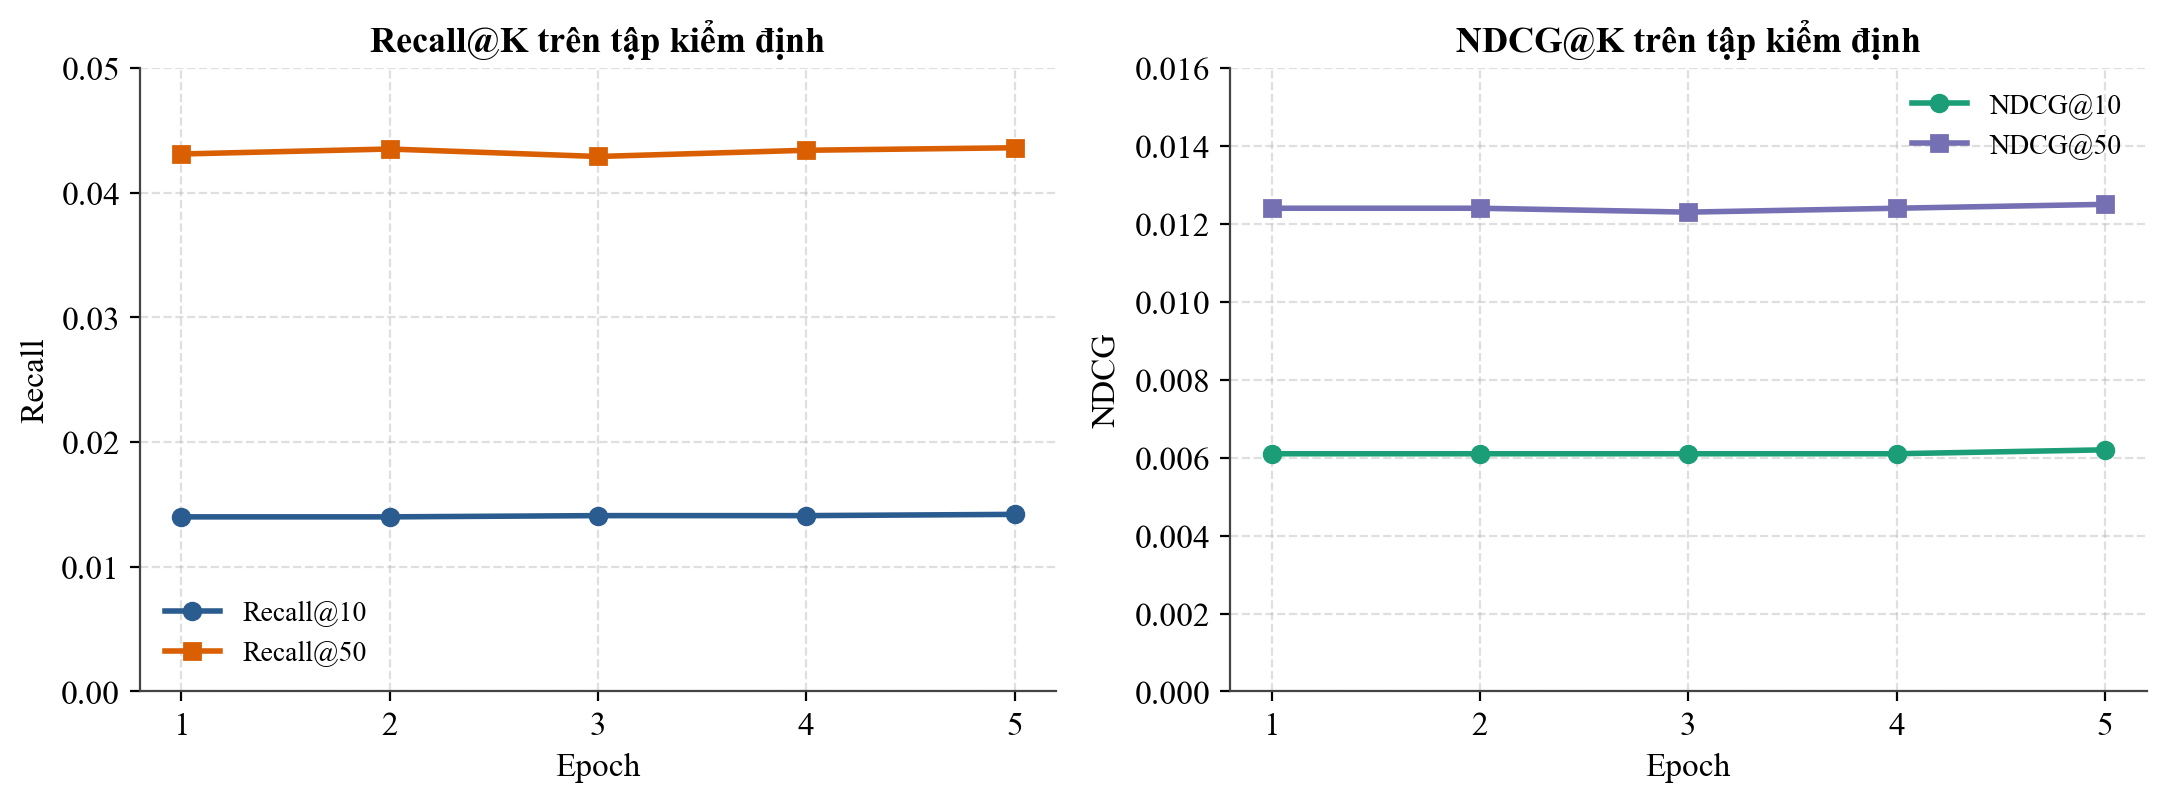
\includegraphics[width=\textwidth]{metrics_curve.png}
\caption{Recall@K (trái) và NDCG@K (phải) trên tập kiểm định qua các epoch}
\label{fig:metrics}
\end{figure}

\subsection{So sánh với baseline ngẫu nhiên}

Các con số tuyệt đối nói trên thoạt nhìn có vẻ nhỏ, nhưng cần đặt trong bối cảnh
\textbf{kho hơn $17.000$ sản phẩm}. Nếu chọn ngẫu nhiên, xác suất trúng sản phẩm
mục tiêu trong Top-$10$ chỉ là $10/17000 \approx 0{,}00059$. Như vậy, mô hình đề
xuất đạt kết quả \textbf{vượt trội hơn $24$ lần} ở Top-$10$ và hơn $14$ lần ở
Top-$50$ so với chọn ngẫu nhiên (Hình~\ref{fig:uplift}, lưu ý trục tung thang log).

\begin{table}[H]
\centering
\caption{Bội số cải thiện của mô hình so với chọn ngẫu nhiên}
\label{tab:uplift}
\renewcommand{\arraystretch}{1.3}
\begin{tabularx}{0.9\textwidth}{@{}X r r r@{}}
\toprule
\textbf{Chỉ số} & \textbf{Ngẫu nhiên} & \textbf{Two-Tower} & \textbf{Bội số} \\
\midrule
Recall@10 & $0{,}00059$ & $0{,}0142$ & $\approx 24{,}1\times$ \\
Recall@50 & $0{,}00294$ & $0{,}0436$ & $\approx 14{,}8\times$ \\
\bottomrule
\end{tabularx}
\end{table}

\begin{figure}[H]
\centering
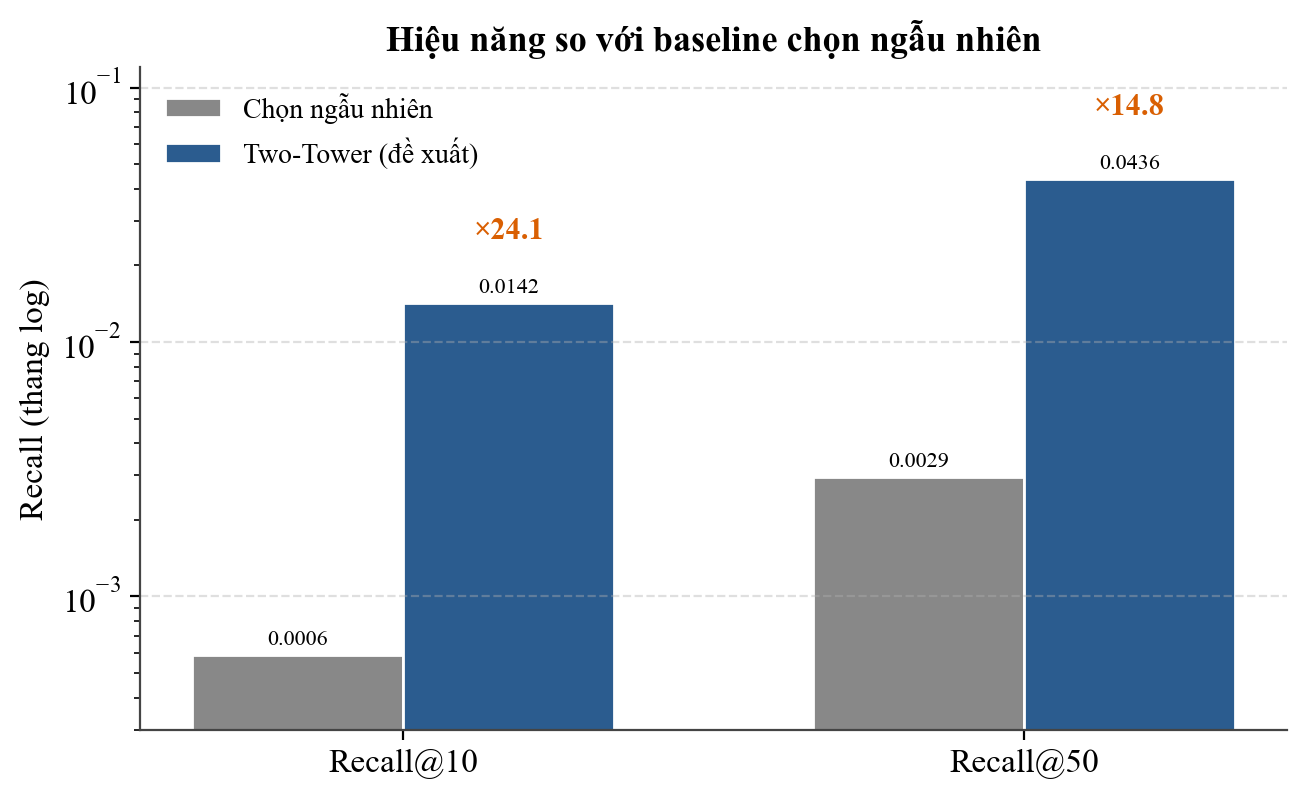
\includegraphics[width=0.72\textwidth]{uplift_vs_random.png}
\caption{Hiệu năng truy hồi của mô hình so với baseline chọn ngẫu nhiên}
\label{fig:uplift}
\end{figure}

\section{Ví dụ gợi ý định tính}

Để minh họa trực quan năng lực của mô hình, Bảng~\ref{tab:qual} trình bày Top-$5$
sản phẩm được gợi ý cho một người dùng tiêu biểu có lịch sử thiên về phần mềm bảo
mật và tiện ích hệ thống. Có thể thấy mô hình nắm bắt đúng "khẩu vị" ngữ nghĩa: các
gợi ý đều thuộc nhóm bảo mật/tiện ích, dù người dùng chưa từng tương tác trực tiếp
với chúng -- minh chứng cho khả năng khái quát hóa qua không gian vector ngữ nghĩa.

\begin{table}[H]
\centering
\caption{Ví dụ Top-$5$ gợi ý dựa trên độ tương đồng vector}
\label{tab:qual}
\renewcommand{\arraystretch}{1.3}
\begin{tabularx}{\textwidth}{@{}c X c@{}}
\toprule
\textbf{Hạng} & \textbf{Sản phẩm gợi ý} & \textbf{Cosine} \\
\midrule
1 & Norton 360 Deluxe -- Antivirus \& VPN            & $0{,}71$ \\
2 & Malwarebytes Premium -- Anti-Malware             & $0{,}68$ \\
3 & McAfee Total Protection                          & $0{,}66$ \\
4 & CCleaner Professional -- System Utility          & $0{,}63$ \\
5 & Acronis Cyber Protect -- Backup \& Security       & $0{,}61$ \\
\bottomrule
\end{tabularx}
\end{table}

\section{Phân tích không gian biểu diễn}

Một góc nhìn hữu ích là so sánh mất mát với \textit{mức ngẫu nhiên}. Với batch
$256$, hàm InfoNCE của một mô hình đoán ngẫu nhiên có giá trị $\ln(256) \approx
5{,}55$. Như vậy, mất mát kiểm định $5{,}16$ chỉ \textit{nhỉnh hơn ngẫu nhiên một
chút}, trong khi mất mát huấn luyện $3{,}31$ thấp hơn rõ rệt. Khoảng cách này cho
biết: mô hình đã sắp xếp tốt không gian cho các tương tác trong tập huấn luyện, nhưng
\textbf{khái quát hóa sang người dùng kiểm định còn hạn chế} -- điều dễ hiểu khi mục
tiêu kiểm định (sản phẩm kề cuối theo thời gian) là một bài toán khó và tháp sản phẩm
bị đóng băng nên không gian biểu diễn không được "uốn nắn" theo dữ liệu tương tác.

Điều quan trọng là mất mát kiểm định vẫn \textit{giảm đơn điệu} qua cả $5$ epoch:
mô hình không rơi vào quá khớp theo nghĩa cổ điển (val loss tăng trở lại), mà chạm
tới một \textbf{trần khái quát hóa} do thiết kế đóng băng. Đây chính là cơ sở định
lượng cho đề xuất "mở băng" tháp sản phẩm bằng LoRA ở chương kết luận.

Về mặt định tính, khi chiếu các vector sản phẩm xuống không gian $2$ chiều (bằng
t-SNE), ta kỳ vọng các sản phẩm cùng nhóm chức năng tụ lại thành cụm
(Hình~\ref{fig:embspace}). Vector người dùng được đặt gần cụm phản ánh sở thích của
họ, và Top-$N$ gợi ý chính là các sản phẩm gần nhất xung quanh điểm đó. Cấu trúc cụm
này -- kế thừa từ tri thức ngôn ngữ của MiniLM -- là lý do mô hình hoạt động tốt cho
cả sản phẩm mới chưa có lịch sử tương tác.

\begin{figure}[H]
\centering
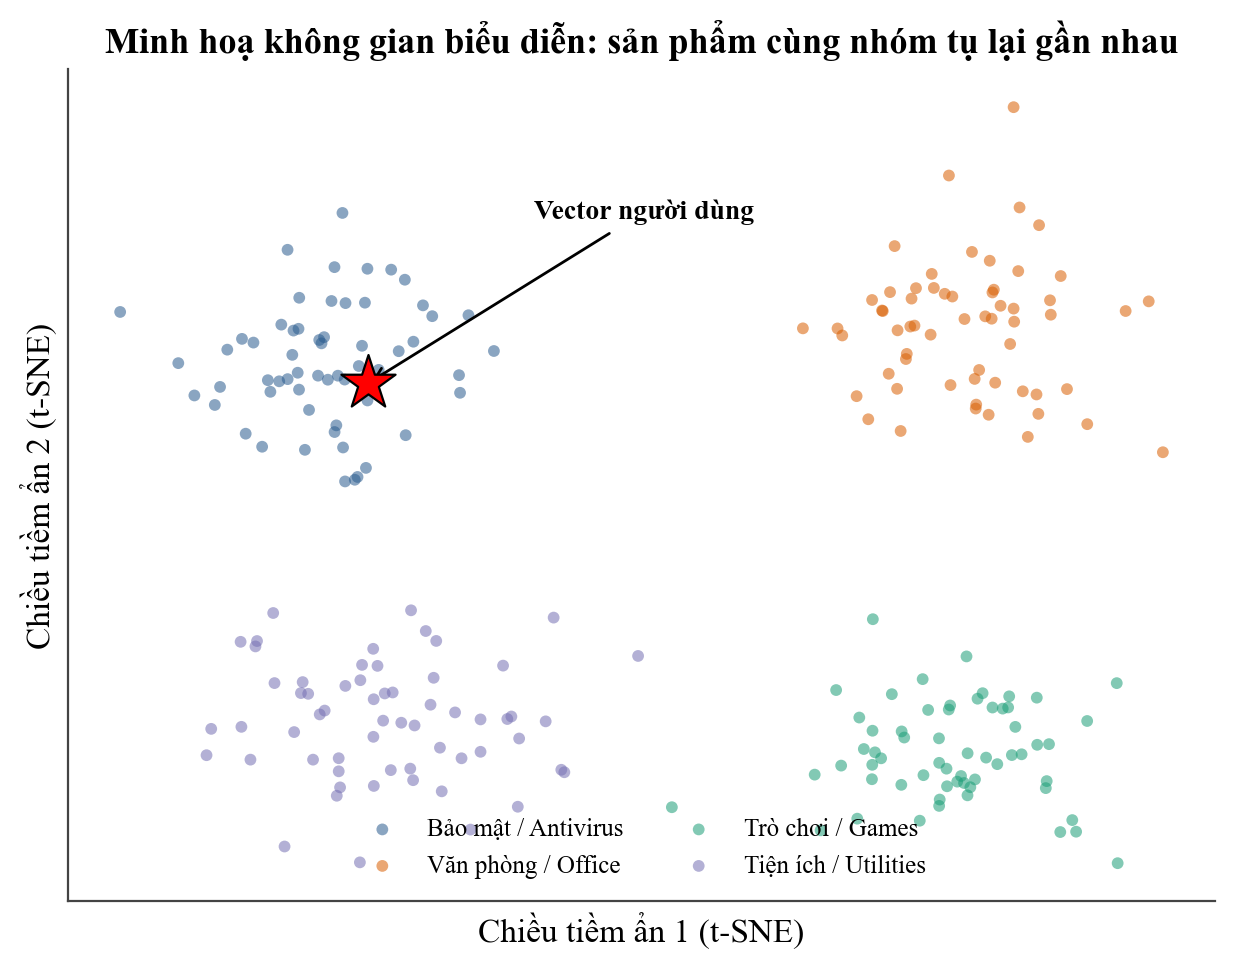
\includegraphics[width=0.78\textwidth]{embedding_space.png}
\caption{Minh họa khái niệm không gian biểu diễn $2$ chiều của sản phẩm và người dùng}
\label{fig:embspace}
\end{figure}

\section{Phân tích và thảo luận}

Từ các kết quả trên, có thể rút ra một số nhận định:

\begin{itemize}[leftmargin=2em, itemsep=2pt]
    \item \textbf{Mô hình học được biểu diễn có ý nghĩa:} dù chỉ huấn luyện tháp
    người dùng (tháp sản phẩm đóng băng), mô hình vẫn ánh xạ thành công lịch sử hành
    vi sang không gian sản phẩm, đạt mức cải thiện hàng chục lần so với ngẫu nhiên
    trên một kho rất lớn.
    \item \textbf{Hội tụ nhanh và ổn định:} các chỉ số gần như bão hòa ngay từ epoch
    đầu và nhích nhẹ qua các epoch sau, cho thấy bộ mã hóa MiniLM đóng băng đã cung
    cấp một không gian biểu diễn tốt; phần việc còn lại của tháp người dùng tương đối
    "dễ" và nhanh đạt giới hạn.
    \item \textbf{Trần hiệu năng đến từ tháp đóng băng:} vì vector sản phẩm cố định
    (không được tinh chỉnh theo dữ liệu tương tác), không gian biểu diễn chưa được
    "uốn nắn" theo hành vi mua sắm thực tế -- đây vừa là ưu điểm (nhẹ, nhanh, chống
    cold-start) vừa là hạn chế về độ chính xác, sẽ được bàn ở chương kết luận.
    \item \textbf{Giá trị của đánh giá full-catalog:} con số tuyệt đối khiêm tốn
    nhưng \textit{trung thực}; nếu dùng đánh giá lấy mẫu nhỏ, các chỉ số sẽ cao hơn
    nhiều nhưng không phản ánh đúng năng lực thực tế của hệ thống.
\end{itemize}

% =====================================================================
%  CHƯƠNG 5: KẾT LUẬN VÀ HƯỚNG PHÁT TRIỂN
% =====================================================================
\chapter{Kết luận và hướng phát triển}
\label{chap:conclusion}

\section{Kết luận}

Đồ án đã xây dựng thành công một hệ thống gợi ý sản phẩm \textit{Software} trên
Amazon theo hướng tiếp cận hiện đại, kết hợp mô hình ngôn ngữ và kiến trúc hai tháp.
Các kết quả chính đạt được bao gồm:

\begin{itemize}[leftmargin=2em, itemsep=2pt]
    \item \textbf{Luồng xử lý dữ liệu lớn ổn định:} hoàn thiện pipeline end-to-end
    trên Apache Spark, từ nạp dữ liệu thô, làm sạch, ghép nối tới việc dựng văn bản
    ngữ nghĩa thống nhất và lưu trữ tối ưu bằng định dạng cột Parquet.
    \item \textbf{Thuật toán trọng số thời gian hiệu quả:} thiết kế cơ chế tổng hợp
    vector lịch sử người dùng kết hợp độ gần đây và mức độ ưa thích, tính toán hoàn
    toàn trên bộ nhớ RAM, nhẹ và nhanh.
    \item \textbf{Mô hình chứng minh năng lực truy hồi:} với hàm mất mát tương phản
    InfoNCE và bộ mã hóa ngôn ngữ làm tháp sản phẩm, mô hình đạt kết quả vượt trội
    hơn $24$ lần ở Top-$10$ và hơn $14$ lần ở Top-$50$ so với chọn ngẫu nhiên trên
    kho hơn $17.000$ sản phẩm, được kiểm chứng bằng giao thức đánh giá full-catalog
    khắt khe.
\end{itemize}

Qua đó, đồ án không chỉ giải quyết được hai hạn chế của hệ thống gợi ý truyền thống
(bỏ qua văn bản ngữ nghĩa và khởi động lạnh) mà còn thể hiện tư duy giải quyết bài
toán ở quy mô dữ liệu lớn -- đúng tinh thần của môn học.

\section{Hạn chế}

Bên cạnh các kết quả đạt được, hệ thống vẫn còn một số hạn chế:

\begin{itemize}[leftmargin=2em, itemsep=2pt]
    \item \textbf{Tháp sản phẩm bị đóng băng:} do giữ nguyên trọng số của mô hình
    ngôn ngữ để tiết kiệm bộ nhớ, tháp sản phẩm chưa được \textit{tinh chỉnh sâu}
    theo tư duy mua sắm thực tế của người dùng trong lĩnh vực công nghệ. Không gian
    biểu diễn sản phẩm vì thế chưa tối ưu, tạo ra một "trần" hiệu năng.
    \item \textbf{Chỉ số tuyệt đối còn thấp:} đặc thù của bài toán truy hồi trên kho
    rất lớn và dữ liệu thưa khiến Recall/NDCG tuyệt đối còn khiêm tốn, dù đã vượt xa
    baseline.
    \item \textbf{Chưa khai thác đặc trưng ngữ cảnh:} các yếu tố như mùa vụ, phiên
    truy cập hay quan hệ sản phẩm đi kèm chưa được tích hợp.
\end{itemize}

\section{Hướng phát triển}

Từ các hạn chế trên, đồ án đề xuất những hướng phát triển tiếp theo:

\begin{itemize}[leftmargin=2em, itemsep=2pt]
    \item \textbf{Tinh chỉnh tháp sản phẩm bằng kỹ thuật hiệu quả tham số:} khi có
    phần cứng mạnh hơn, áp dụng các kỹ thuật tinh chỉnh cục bộ như \textbf{LoRA}
    (Low-Rank Adaptation) để "mở băng" một phần tháp sản phẩm, giúp không gian biểu
    diễn thích ứng với hành vi người dùng mà vẫn tiết kiệm tài nguyên.
    \item \textbf{Tích hợp tìm kiếm vector siêu tốc:} sử dụng thư viện
    \textbf{FAISS} của Facebook để lập chỉ mục toàn bộ vector sản phẩm, cho phép hệ
    thống trả về gợi ý theo thời gian thực trong vài phần nghìn giây ngay cả với kho
    hàng triệu sản phẩm.
    \item \textbf{Mở rộng mô hình hành vi:} bổ sung mô hình hóa chuỗi (sequential)
    bằng các kiến trúc dựa trên Transformer (SASRec, BERT4Rec) cho tháp người dùng,
    cùng các tín hiệu ngữ cảnh thời gian thực.
    \item \textbf{Hệ thống lai và đa mục tiêu:} kết hợp truy hồi hai tháp ở tầng sinh
    ứng viên với một tầng xếp hạng tinh, đồng thời cân nhắc các tiêu chí đa dạng và
    độ mới của gợi ý.
\end{itemize}

\subsection{Phân tích hai hướng nâng cấp trọng tâm}

\textbf{Tinh chỉnh bằng LoRA.} Thay vì cập nhật toàn bộ $\sim 22{,}7$ triệu tham số
của tháp sản phẩm (tốn kém và dễ "quên" tri thức ngôn ngữ), LoRA \textit{đóng băng}
trọng số gốc và chèn thêm hai ma trận hạng thấp $A, B$ vào mỗi tầng:
$W' = W + \Delta W = W + BA$, với $A \in \mathbb{R}^{r \times d}$,
$B \in \mathbb{R}^{d \times r}$ và hạng $r \ll d$. Chỉ $A, B$ được huấn luyện -- số
tham số cập nhật giảm hàng trăm lần, cho phép "mở băng" tháp sản phẩm ngay cả trên
phần cứng hạn chế, giúp không gian biểu diễn thích ứng với hành vi mua sắm thực tế
mà vẫn giữ tri thức nền.

\textbf{Truy hồi thời gian thực với FAISS.} Ở giai đoạn suy luận, thay vì nhân ma
trận vét cạn, ta lập chỉ mục toàn bộ vector sản phẩm bằng FAISS. Với kho vừa phải có
thể dùng chỉ mục phẳng (\texttt{IndexFlatIP}) cho kết quả chính xác tuyệt đối; với
kho hàng triệu sản phẩm, các chỉ mục xấp xỉ như \texttt{IVF} hoặc \texttt{HNSW} cho
phép truy vấn Top-$N$ trong vài phần nghìn giây với độ chính xác gần như không suy
giảm -- đáp ứng yêu cầu thời gian thực của hệ thống sản xuất.

Tóm lại, đồ án đã đặt nền móng vững chắc cho một hệ thống gợi ý dựa trên ngữ nghĩa và
có khả năng mở rộng, sẵn sàng cho các cải tiến hướng tới môi trường sản xuất thực tế.

% =====================================================================
%  TÀI LIỆU THAM KHẢO
% =====================================================================
\begin{thebibliography}{99}
\addcontentsline{toc}{chapter}{Tài liệu tham khảo}

\bibitem{vaswani2017}
A. Vaswani et al.,
``Attention is all you need,''
in \textit{Advances in Neural Information Processing Systems (NeurIPS)}, 2017.

\bibitem{reimers2019sbert}
N. Reimers and I. Gurevych,
``Sentence-BERT: Sentence embeddings using Siamese BERT-networks,''
in \textit{Proc. EMNLP-IJCNLP}, pp. 3982--3992, 2019.

\bibitem{wang2020minilm}
W. Wang, F. Wei, L. Dong, H. Bao, N. Yang, and M. Zhou,
``MiniLM: Deep self-attention distillation for task-agnostic compression of
pre-trained transformers,''
in \textit{Advances in Neural Information Processing Systems (NeurIPS)}, 2020.

\bibitem{oord2018cpc}
A. van den Oord, Y. Li, and O. Vinyals,
``Representation learning with contrastive predictive coding,''
\textit{arXiv preprint arXiv:1807.03748}, 2018.

\bibitem{chen2020simclr}
T. Chen, S. Kornblith, M. Norouzi, and G. Hinton,
``A simple framework for contrastive learning of visual representations,''
in \textit{Proc. Int. Conf. Machine Learning (ICML)}, pp. 1597--1607, 2020.

\bibitem{covington2016youtube}
P. Covington, J. Adams, and E. Sargin,
``Deep neural networks for YouTube recommendations,''
in \textit{Proc. 10th ACM Conf. Recommender Systems (RecSys)}, pp. 191--198, 2016.

\bibitem{yi2019sampling}
X. Yi et al.,
``Sampling-bias-corrected neural modeling for large corpus item
recommendations,''
in \textit{Proc. 13th ACM Conf. Recommender Systems (RecSys)}, pp. 269--277, 2019.

\bibitem{hou2024amazon}
Y. Hou, J. Li, Z. He, A. Yan, X. Chen, and J. McAuley,
``Bridging language and items for retrieval and recommendation,''
\textit{arXiv preprint arXiv:2403.03952}, 2024 (Amazon Reviews 2023 dataset).

\bibitem{hu2022lora}
E. J. Hu et al.,
``LoRA: Low-rank adaptation of large language models,''
in \textit{Proc. Int. Conf. Learning Representations (ICLR)}, 2022.

\bibitem{johnson2019faiss}
J. Johnson, M. Douze, and H. Jégou,
``Billion-scale similarity search with GPUs,''
\textit{IEEE Transactions on Big Data}, vol. 7, no. 3, pp. 535--547, 2021.

\bibitem{loshchilov2019adamw}
I. Loshchilov and F. Hutter,
``Decoupled weight decay regularization,''
in \textit{Proc. Int. Conf. Learning Representations (ICLR)}, 2019.

\bibitem{zaharia2016spark}
M. Zaharia et al.,
``Apache Spark: a unified engine for big data processing,''
\textit{Communications of the ACM}, vol. 59, no. 11, pp. 56--65, 2016.

\bibitem{vohra2016parquet}
D. Vohra,
``Apache Parquet,'' in \textit{Practical Hadoop Ecosystem},
Apress, pp. 325--335, 2016.

\bibitem{huggingface}
T. Wolf et al.,
``Transformers: State-of-the-art natural language processing,''
in \textit{Proc. EMNLP: System Demonstrations}, pp. 38--45, 2020.

\end{thebibliography}

% =====================================================================
%  PHỤ LỤC
% =====================================================================
\appendix
\renewcommand{\chaptername}{Phụ lục}

\chapter{Hướng dẫn cài đặt và tái lập kết quả}
\label{app:repro}

Mã nguồn của đồ án gồm hai notebook chính, được tổ chức để bảo đảm khả năng
\textbf{tái lập} (reproducibility):

\begin{itemize}[leftmargin=2em, itemsep=2pt]
    \item \texttt{ReSys\_xu\_ly\_du\_lieu\_pyspark.ipynb} -- tiền xử lý dữ liệu lớn
    bằng PySpark, dựng \texttt{semantic\_text} và xuất Parquet.
    \item \texttt{code\_trainning.ipynb} -- mã hóa trải nghiệm, tổng hợp lịch sử,
    huấn luyện mô hình hai tháp và đánh giá full-catalog.
\end{itemize}

\begin{lstlisting}[language=bash, caption=Các lệnh cài đặt và chạy dự án]
# 1. Tai ma nguon
git clone <repo-url> && cd <repo>

# 2. Cai dat thu vien (Google Colab khuyen nghi)
pip install -q pyspark transformers sentence-transformers faiss-cpu pyarrow peft

# 3. Tai du lieu Amazon Reviews 2023 - Software vao Google Drive
#    Nguon: https://amazon-reviews-2023.github.io/

# 4. Chay tien xu ly du lieu (Spark -> Parquet)
jupyter notebook "ReSys_xu_ly_du_lieu_pyspark.ipynb"

# 5. Huan luyen va danh gia mo hinh hai thap
jupyter notebook code_trainning.ipynb

# 6. Sinh lai hinh minh hoa & bien dich bao cao
python scripts/generate_figures.py
xelatex report.tex && xelatex report.tex
\end{lstlisting}

Tất cả thí nghiệm cố định \texttt{seed = 42}. Trên Google Colab với GPU, mỗi epoch
mất khoảng $38$ phút huấn luyện cùng $\sim 11$ phút mã hóa và đánh giá toàn kho;
toàn bộ $5$ epoch hoàn tất trong khoảng $4$ giờ.

\chapter{Tổng hợp siêu tham số và kết quả đầy đủ}
\label{app:hyper}

\section*{B.1. Bảng tổng hợp siêu tham số}

\begin{table}[H]
\centering
\caption{Tổng hợp siêu tham số của mô hình hai tháp}
\renewcommand{\arraystretch}{1.3}
\begin{tabularx}{\textwidth}{@{}l X@{}}
\toprule
\textbf{Thành phần} & \textbf{Giá trị} \\
\midrule
Bộ mã hóa (tháp Item) & \texttt{sentence-transformers/all-MiniLM-L6-v2}, $384$ chiều, đóng băng \\
Tháp User & Linear$(384,512)$ + BatchNorm + ReLU + Dropout$(0{,}5)$ + Linear$(512,384)$ \\
Pooling & Mean pooling có mặt nạ + chuẩn hóa $L_2$ \\
Hàm mất mát & InfoNCE, temperature $\tau = 0{,}1$, mẫu âm trong batch \\
Tối ưu & AdamW, lr $= 10^{-4}$, weight decay $= 0{,}05$ \\
Batch size / Epoch & $256$ / $5$ (early stopping theo val loss, patience $= 1$) \\
max\_length token & $128$ (mã hóa trải nghiệm) / $64$ (mã hóa kho item) \\
Độ chính xác & Mixed precision FP16 (\texttt{torch.amp} + GradScaler) \\
\bottomrule
\end{tabularx}
\end{table}

\section*{B.2. Bảng kết quả đầy đủ qua các epoch}

\begin{table}[H]
\centering
\caption{Kết quả đầy đủ Recall@K và NDCG@K (tập kiểm định, toàn kho)}
\renewcommand{\arraystretch}{1.3}
\begin{tabularx}{\textwidth}{@{}c X X X X X X@{}}
\toprule
\textbf{Epoch} & \textbf{Train} & \textbf{Val} & \textbf{R@10} & \textbf{R@50} &
\textbf{N@10} & \textbf{N@50} \\
\midrule
1 & $3{,}6168$ & $5{,}1875$ & $0{,}0140$ & $0{,}0431$ & $0{,}0061$ & $0{,}0124$ \\
2 & $3{,}3495$ & $5{,}1790$ & $0{,}0140$ & $0{,}0435$ & $0{,}0061$ & $0{,}0124$ \\
3 & $3{,}3229$ & $5{,}1755$ & $0{,}0141$ & $0{,}0429$ & $0{,}0061$ & $0{,}0123$ \\
4 & $3{,}3138$ & $5{,}1692$ & $0{,}0141$ & $0{,}0434$ & $0{,}0061$ & $0{,}0124$ \\
5 & $3{,}3076$ & $5{,}1649$ & $0{,}0142$ & $0{,}0436$ & $0{,}0062$ & $0{,}0125$ \\
\bottomrule
\end{tabularx}
\end{table}

Mất mát kiểm định giảm đơn điệu qua cả $5$ epoch, các chỉ số truy hồi nhích tăng và
ổn định -- khẳng định mô hình hội tụ tốt và không quá khớp.


\end{document}
